\documentclass[12pt,twoside]{Book} 
% \usepackage[a4paper,tmargin=1.5cm, bmargin=2cm, lmargin=1.5cm, rmargin=1.5cm]{geometry}
\usepackage[a4paper,tmargin=2cm, bmargin=2.5cm, lmargin=3.5cm, rmargin=2.0cm]{geometry}
\usepackage{color,calc,graphicx,soul,fourier}  
\usepackage{graphicx}
\usepackage{amsmath,amssymb,latexsym,amsfonts, bbm,mathtools, enumitem,esvect,commath,pifont}
\usepackage[backend=biber, style=alphabetic, sorting=ynt]{biblatex}
\usepackage{fourier}
\usepackage{titling}
\usepackage{longtable}
\usepackage{gensymb}
% \usepackage[utf8]{vietnam}
\usepackage{afterpage}
\usepackage{enumitem}
\usepackage{xparse}
\usepackage{tabvar}
\usepackage{titlesec} 
\usepackage{lipsum}
\usepackage{tikz,pgf,tkz-tab}
\usepackage{multicol}
\usepackage{pdfpages}
\usepackage{fancyhdr}
\usepackage{xparse}
\usepackage{hyperref}
\usepackage{chngcntr}
\usepackage{listings}
\usepackage[absolute,overlay]{textpos}
\usepackage[lined,boxed,commentsnumbered]
\definecolor{codegreen}{rgb}{0,0.6,0}
\definecolor{codegray}{rgb}{0.5,0.5,0.5}
\definecolor{codepurple}{rgb}{0.58,0,0.82}
%\definecolor{backcolour}{rgb}{0,0.95,0.92}
%% Remember to load babel before loading this package or define the command \abstractname!
	  
\lstdefinestyle{mystyle}{
    backgroundcolor=\color{white},   
    commentstyle=\color{codegreen},
    keywordstyle=\color{magenta},
    numberstyle=\tiny\color{codegray},
    stringstyle=\color{codepurple},
    basicstyle=\ttfamily\footnotesize,
    breakatwhitespace=false,         
    breaklines=true,                 
    captionpos=b,                    
    keepspaces=true,                 
    numbers=left,                    
    numbersep=5pt,                  
    showspaces=false,                
    showstringspaces=false,
    showtabs=false,                  
    tabsize=2
}

\lstset{style=mystyle}
\usepackage{hyperref}
\hypersetup{
    colorlinks=true,
    linkcolor=blue,
    filecolor=magenta,      
    urlcolor=cyan,
    pdftitle={Overleaf Example},
    pdfpagemode=FullScreen,
}
\urlstyle{same}
\pagestyle{fancy}
\lhead[]{}\chead[]{}\rhead[]{}
\lfoot[\sl Page \thepage]{
    \it Logic Design Project
    \hfil 
}
\cfoot[]{}
\rfoot[\it HCMUT - Computer Engineering]{\sl Page \thepage}
\renewcommand{\headrulewidth}{0pt}
\renewcommand{\footrulewidth}{1pt}  
\setlength{\parindent}{0pt}
\newcommand{\debugline}{\vspace{-0.5cm}\phantom{Debug error no line to end}}
\newcommand\blankpage{%
    \null
    \thispagestyle{empty}%
    \addtocounter{page}{0}%
    \newpage}

\newcommand*{\TitleFont}{%
      \usefont{\encodingdefault}{\rmdefault}{b}{n}%
      \fontsize{40pt}{50pt}%
      \selectfont}

\titleformat{\chapter}[display]
  {\bfseries\Huge}
  {\filright\MakeUppercase{\chaptertitlename} \Huge\thechapter}
  {2ex}
  {\titlerule\vspace{1ex}\filleft}
  [\vspace{1ex}\titlerule]
  
\addbibresource{references.bib} %Imports bibliography file

% Input definition for questions


\counterwithin*{section}{chapter}
\counterwithin*{subsection}{section}
\counterwithin*{subsubsection}{subsection}

\newbox\allanswers
\setbox\allanswers=\hbox{}
\newcommand{\addanswer}[2]{%
  \global\setbox\allanswers=\hbox{\unhbox\allanswers #1.~#2\quad}%
}
\newcommand{\showanswers}{%
  \vfill
  \begin{center}
    ................
  \end{center}
  \noindent\unhbox\allanswers
}

\begin{document}
\begin{titlepage}
\begin{center}
\textcolor{black}{\textbf{\large VIETNAM NATIONAL UNIVERSITY HO CHI MINH CITY}} \\
\textcolor{black}{\textbf{ \large HO CHI MINH CITY UNIVERSITY OF TECHNOLOGY}}\\
\textcolor{black}{\textbf{\large FACULTY OF COMPUTER SCIENCE AND ENGINEERING}}\\
-----------------------------------------
\end{center}

\vspace{1cm}

\begin{figure}[h!]
\begin{center}

\includegraphics[width=4.7cm]{source/picture/3_Logo_BK.png}
\end{center}
\end{figure}

\vspace{0.7cm}


\begin{center}
\begin{tabular}{c}
	\multicolumn{1}{c}{\textcolor{black}{\textbf{{\large LOGIC DESIGN PROJECT REPORT}}}}\\
    ~~\\
    \textbf{{\textcolor{black}{\LARGE FPGA-BASED IMPLEMENTATION FOR }}}\\
    
    \textbf{\LARGE MACHINE LEARNING APPLICATION}\\
    \textbf{\LARGE AND CONVOLUTION COMPUTING SIMULATION}\\
    \\
    \large Major: Computer Engineering
\end{tabular}
\end{center}

\vspace{1.2cm}
\hspace{5.7cm}\textbf{LOGIC DESIGN PROJECT COMMITEE 3}
\begin{table}[h]
\begin{tabular}{rll}
\hspace{5cm}
& \textbf{INSTRUCTOR:} &\textbf{PHAM QUOC CUONG}\\
& & \textbf{PHAM DINH TRUNG}\\
\\
& \textbf{STUDENTS:} & \textbf{LE NGOC MINH THU }\\ 
& &\textbf{BUI ANH KHOA}\\
& &\textbf{NGUYEN PHAN ANH TUAN }

\end{tabular}
\end{table}
\vspace{1cm}
\begin{center}
{\textcolor{black}{\footnotesize Winter Semester, AY 2022-2023}}
\end{center}
\end{titlepage}
\newpage

\tableofcontents

\clearpage
\vspace{2cm}
\textbf{Member list}
\begin{center}
\begin{tabular}{|c|c|c|c|}
\hline
\textbf{No.} & \textbf{Fullname} & \textbf{Student ID} & \textbf{Email}\\
\hline 
%%%%%Student 1%%%%%%%%%%
 & &  &  \\
{1} & {Huynh Trung Nhat} & {2053294} &{nhat.huynhtrung328@hcmut.edu.vn}\\
 & &  &  \\
\hline 
%%%%%Student 2%%%%%%%%%%
 & &  &  \\
{2} & {Do Huu Thanh Thien} & {2053453} &{thien.dh412@hcmut.edu.vn}\\
 & &  &  \\
\hline 

\end{tabular}
\end{center}
\chap{ Switches, Lights, and Multiplexers}
\section{Part I }
\begin{itemize}
    \item [] \textbf{REQUIREMENT}
        \begin{enumerate}
            \item Create a new Quartus project for your circuit. Select the target chip that corresponds to your DE-series board. Refer to Table 1 for a list of devices.
            \item Create a Verilog module for the code in Figure 1 and include it in your project.
            \item Include in your project the required pin assignments for your DE-series board, as discussed above. Compile the project.
            \item Download the compiled circuit into the FPGA chip by using the Quartus Programmer tool (the procedure for using the Programmer tool is described in the tutorial Quartus Introduction). Test the functionality of the circuit by toggling the switches and observing the LEDs.
        \end{enumerate}
    \item [] \textbf{SOLUTION}
            \begin{lstlisting}[language=verilog]
module part2(out, X, Y,S);
    output	[3:0]out;
    input		[3:0]X,Y;
    input		S;
    
    assign out = ({4{S}}&X) | ({4{~S}}&Y);
endmodule
            \end{lstlisting}
             \begin{figure}[h]
                \centering
                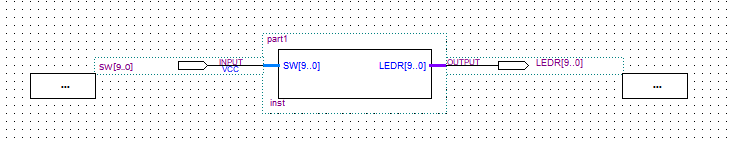
\includegraphics[scale = 0.9]{source/picture/Lab1/Lab1_1.png}
                \caption{Schematic for part 1}
            \end{figure}
\end{itemize}
\clearpage
\section{Part II }
\begin{itemize}
    \item [] \textbf{REQUIREMENT}
        \begin{enumerate}
            \item Create a new Quartus project for your circuit.
            \item Include your Verilog file for the four-bit wide 2-to-1 multiplexer in your project. Use switch $SW_9$ as the s input, switches $SW_{3-0}$ as the X input and $SW_{7-4}$ as the Y input. Display the value of the input s on $LEDR_9$, connect the output M to $LEDR_{3-0}$, and connect the unused LEDR lights to the constant value 0.
            \item Include in your project the required pin assignments for your DE-series board. As discussed in Part I, these assignments ensure that the ports of your Verilog code will use the pins on the FPGA chip that are connected to the SW switches and LEDR lights.
            \item Compile the project, and then download the resulting circuit into the FPGA chip. Test the functionality of the four-bit wide 2-to-1 multiplexer by toggling the switches and observing the LEDs
        \end{enumerate}
    \item [] \textbf{SOLUTION}
        \begin{lstlisting}[language= verilog]
module part2(out, X, Y,S);
	output	[3:0]out;
	input		[3:0]X,Y;
	input		S;
	
	assign out = ({4{S}}&X) | ({4{~S}}&Y);
	
endmodule
        \end{lstlisting}
        \begin{figure}[h]
            \centering
            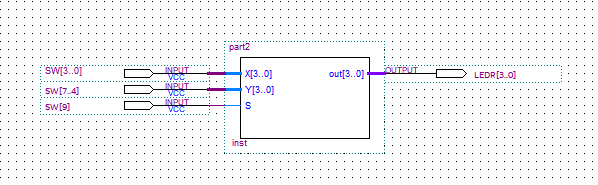
\includegraphics[scale =0.9]{source/picture/Lab1/Lab1_2.png}
            \caption{Schematic for part 2}
        \end{figure}
\end{itemize}
\clearpage
\section{Part III }
\begin{itemize}
    \item [] \textbf{REQUIREMENT}
        \begin{enumerate}
            \item Create a new Quartus project for your circuit.
            \item Create a Verilog module for the two-bit wide 4-to-1 multiplexer. Connect its select inputs to switches $SW_{9-8}$, and use switches $SW_{7-0}$ to provide the four 2-bit inputs U to X. Connect the output M to the red lights $LEDR_{1-0}$.
            \item Include in your project the required pin assignments for your DE-series board. Compile the project.
            \item Download the compiled circuit into the FPGA chip. Test the functionality of the two-bit wide 4-to-1 multiplexer by toggling the switches and observing the LEDs. Ensure that each of the inputs U to X can be properly selected as the output M.
        \end{enumerate}
    \item [] \textbf{SOLUTITON}
        \begin{lstlisting}[language = verilog]
module part3(M,U,V,W,X,S_1,S_0);
    input 	[1:0]U,V,W,X;
    input		S_1,S_0;
    output	[1:0]M;
    
    assign 	M= ({2{S_0&S_1}}&X)|
                    ({2{~S_0&S_1}}&W)|
                    ({2{S_0&~S_1}}&V)|
                    ({2{~S_0&~S_1}}&U);
	
endmodule
        \end{lstlisting}
        \begin{figure}[h]
            \centering
            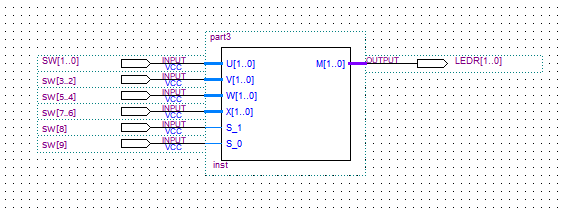
\includegraphics[width = \textwidth]{source/picture/Lab1/Lab1_3.png}
            \caption{Schemactic for part 3}
        \end{figure}
    
\end{itemize}
\clearpage
\section{Part IV }
\begin{itemize}
    \item [] \textbf{REQUIREMENT}
    \begin{enumerate}
        \item The objective of this part is to display a character on a 7-segment display. This decoder produces seven outputs that are used to display a character on a 7-segment display. Table 2 lists the characters that should be displayed for each valuation of c1c0 for your DE-series board.
        \item Note that in some cases the ‘blank’ character is selected for code 11. The seven segments in the display are identified by the indices 0 to 6 shown in the figure. Each segment is illuminated by driving it to the logic value 0. You are to write a Verilog module that implements logic functions to activate each of the seven segments.
    \end{enumerate}    
        \begin{figure}[h]
            \centering
            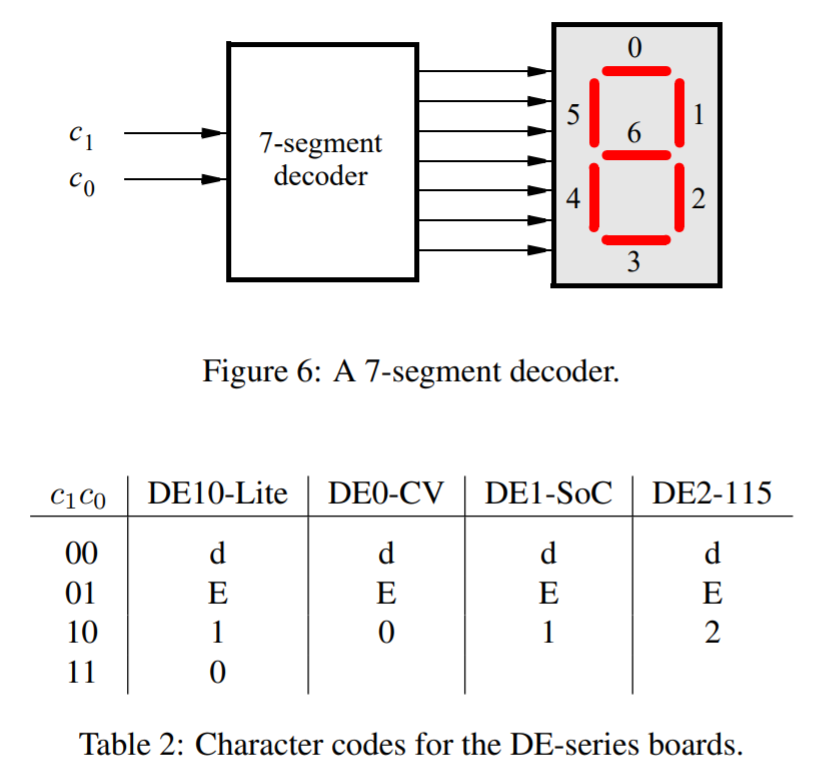
\includegraphics[scale =0.4]{source/picture/Lab1/1-4.png}
        \end{figure}
    \item [] \textbf{SOLUTION}
        \begin{lstlisting} [language = verilog]
module  part4(OUT,C_IN);
    input 	[1:0]C_IN;
    output	[6:0]OUT;
    
    assign 	OUT = (C_IN==0) ? 7'b0100001: 
                  (C_IN==1) ? 7'b0000110: 
                  (C_IN==2) ? 7'b0100100:7'b1111011;
endmodule
        \end{lstlisting}
        \begin{figure}[h]
            \centering
            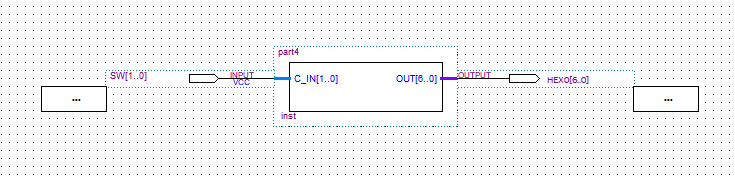
\includegraphics[width=\textwidth]{source/picture/Lab1/Lab1_4.png}
            \caption{Schemtatic for part 4}
        \end{figure}
\end{itemize}

\clearpage
\section{Part V }
\begin{itemize}
    \item [] \textbf{REQUIREMENT}
        \begin{enumerate}
            \item Consider the circuit shown in Figure 7. It uses a two-bit wide 4-to-1 multiplexer to enable the selection of four characters that are displayed on a 7-segment display. Using the 7-segment decoder from Part IV this circuit can display the characters d, E, 0, 1, 2, or 'blank' depending on your DE-series board. The character codes are set according to Table 2 by using the switches SW7-0, and a specific character is selected for display by setting the switches $SW_{9-8}$.
            \item Note that we have used the circuits from Parts III and IV as subcircuits in this code. The purpose of your circuit is to display any word on the four 7-segment displays that is composed of the characters in Table 2, and be able to rotate this word in a circular fashion across the displays when the switches SW9-8 are toggled. As an example, if the displayed word is dE10, then your circuit should produce the output patterns illustrated in Table 3.
        \end{enumerate}
        \begin{figure}[h]
            \centering
            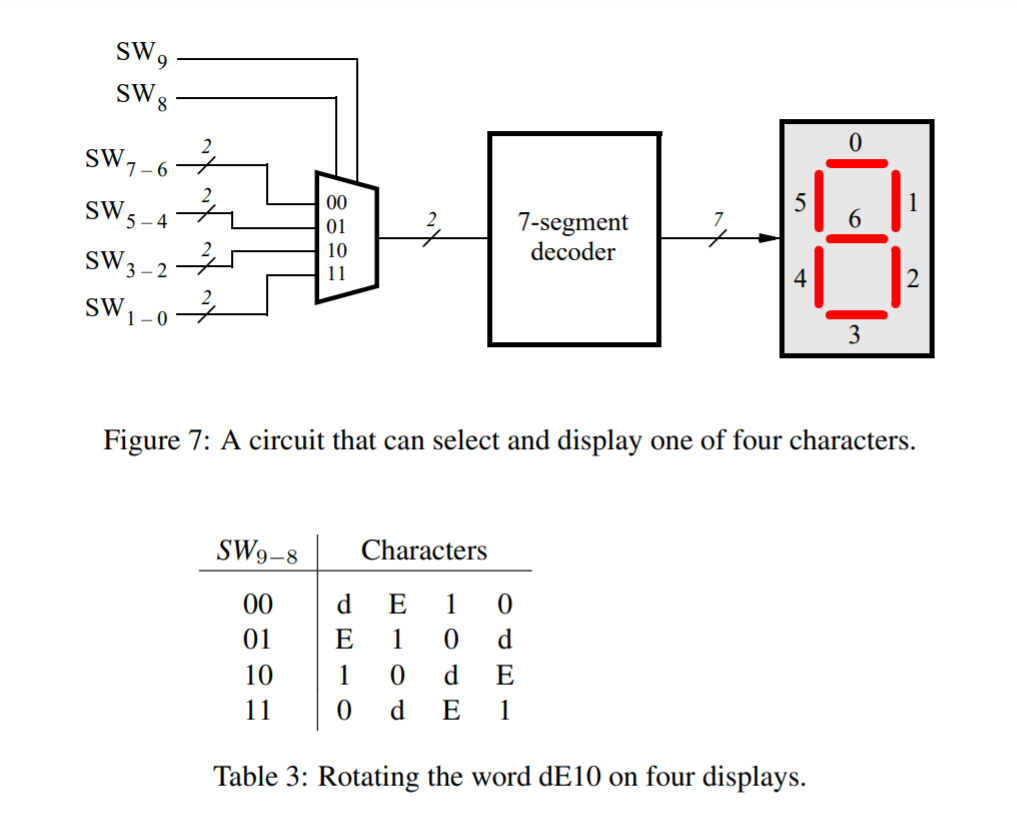
\includegraphics[scale =0.40]{source/picture/Lab1/1-5.png}
        \end{figure}
    \item [] \textbf{SOLUTION} In this part of Lab 1, we reuse part 3 and part 4  block to implement the circuit. 
        \begin{itemize}
            \item [] Part 3 block with 4 fix input and Pin $S_0, S_1$ to select the input
            \item [] Part 4 block use the output of the part 3 as the input and generate signal for four 7-segment leds in DE2i-board.
        \end{itemize}
         
\end{itemize}
\clearpage
\begin{figure}[h]
    \centering
    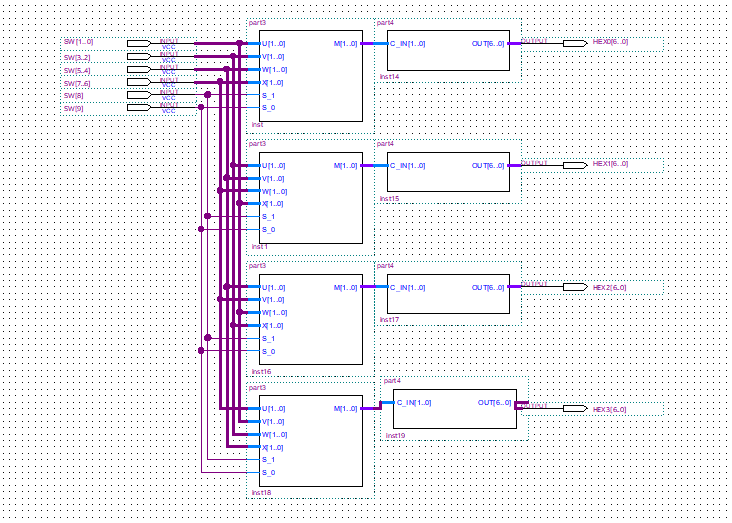
\includegraphics[width=\textwidth]{source/picture/Lab1/Lab1_5.png}
    \caption{Schematic for part 5}
\end{figure}
\clearpage

\section{Part VI }
\begin{itemize}
    \item [] \textbf{REQUIREMENT}
        \begin{enumerate}
            \item Extend your design from Part V so that is uses all 7-segment displays on your DE-series board. Your circuit needs to display a three- or four-letter word, corresponding to Table 2, using 'blank' characters for unused displays. Implement rotation of this word from right-to-left as indicated in Table 4 and Table 5. 
            \item Note that for the DE10-Lite you will need to use 3-bit codes for your characters, because five characters are needed when including the 'blank' character (your 7-segment decoder will have to use 3-bit codes, and you will need to use 3-bit wide 6-to-1 multiplexers). 
        \end{enumerate}
    \item [] \textbf{SOLUTION}
        \begin{lstlisting}[language=Verilog]
module part6(SW,HEX0, HEX1, HEX2, HEX3, HEX4, HEX5, HEX6, HEX7);
	input 	[2:0]SW;
	output 	[6:0]HEX0,HEX1,HEX2, HEX3, HEX4, HEX5, HEX6, HEX7;
	wire		[55:0]hex0,hex1,hex2,hex3,hex4,hex5,hex6,hex7;
	wire		[55:0]temp;

	assign hex0 = {7'b1111111,7'b1111111,7'b1111111,7'b1111111,7'b0100001,7'b0000110,7'b1111001,7'b1111111};
	assign hex1 = {7'b1111111,7'b1111111,7'b1111111,7'b0100001,7'b0000110,7'b1111001,7'b1111111,7'b1111111};
	assign hex2 = {7'b1111111,7'b1111111,7'b0100001,7'b0000110,7'b1111001,7'b1111111,7'b1111111,7'b1111111};
	assign hex3 = {7'b1111111,7'b0100001,7'b0000110,7'b1111001,7'b1111111,7'b1111111,7'b1111111,7'b1111111};
	assign hex4 = {7'b0100001,7'b0000110,7'b1111001,7'b1111111,7'b1111111,7'b1111111,7'b1111111,7'b1111111};
	assign hex5 = {7'b0000110,7'b1111001,7'b1111111,7'b1111111,7'b1111111,7'b1111111,7'b1111111,7'b0100001};
	assign hex6 = {7'b1111001,7'b1111111,7'b1111111,7'b1111111,7'b1111111,7'b1111111,7'b0100001,7'b0000110};
	assign hex7 = {7'b1111111,7'b1111111,7'b1111111,7'b1111111,7'b1111111,7'b0100001,7'b0000110,7'b1111001};
	
	assign temp = (SW==0)?hex0: 
					  (SW==1)?hex1:
					  (SW==2)?hex2:
					  (SW==3)?hex3:
					  (SW==4)?hex4:
					  (SW==5)?hex5:
					  (SW==6)?hex6:hex7;
					  
	assign HEX0 = temp[6:0];
	assign HEX1 = temp[13:7];
	assign HEX2 = temp[20:14];
	assign HEX3 = temp[27:21];
	assign HEX4 = temp[34:28];
	assign HEX5 = temp[41:35];
	assign HEX6 = temp[48:42];
	assign HEX7 = temp[55:49];
	
endmodule
    \end{lstlisting}
\end{itemize}

\clearpage



\begin{figure}[h]
    \centering
    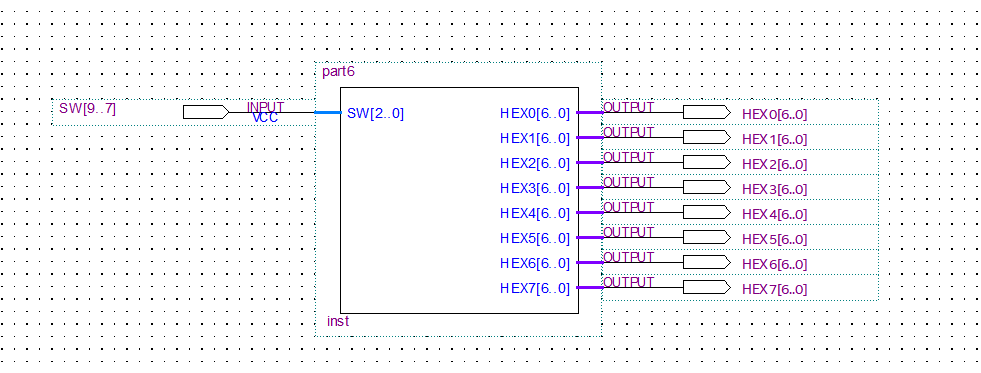
\includegraphics[width = \textwidth]{source/picture/Lab1/Lab1_6.png}
    \caption{Schematic for part 6}
\end{figure}

\begin{figure}[h]
    \centering
    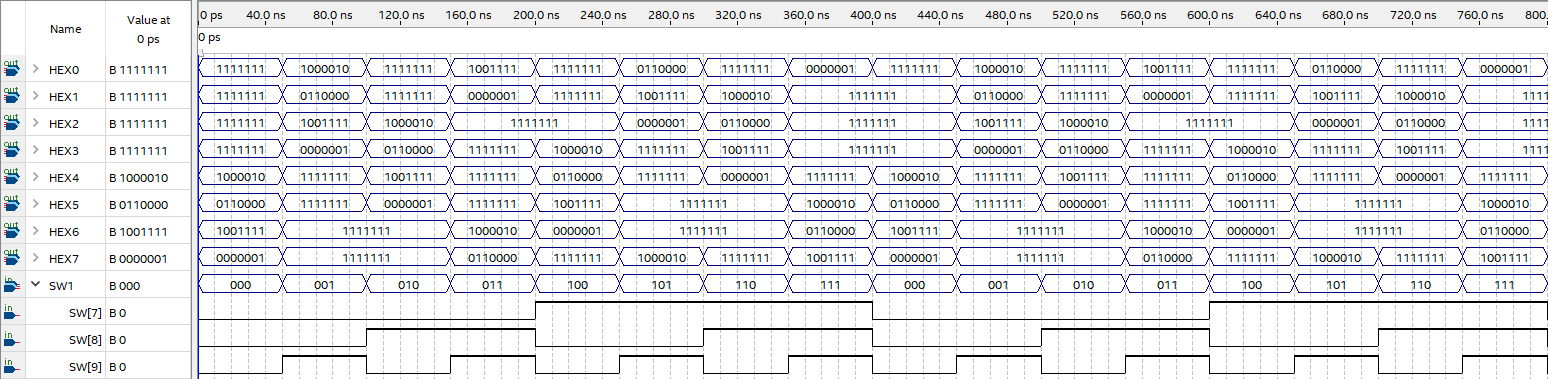
\includegraphics[scale = 0.40]{source/picture/Lab1/Lab1_wave.png}
    \caption{Simulation Result}
\end{figure}
\chap{Numbers and Displays}
\section{Introduction}
This is an exercise in designing combinational circuits that can perform binary-to-decimal number conversion and binary-coded-decimal (BCD) addition.\\
In previous parts, we design and implemented:
\begin{itemize}
    \item Two 7-segment displays inputed by the switches $SW_{7-0}$.
    \item Two-digit decimal represented by 7-segment displays,inputed by the switches $SW_{3-0}$(includes a comparator).
    \item full adder.
    \item Circuit that adds the two BCD digits.
\end{itemize}
\section{Part II}
\begin{itemize}
    \item [] \textbf{REQUIREMENT}
        \begin{enumerate}
            \item You are to design a circuit that converts a four-bit binary number $V = v_3v_2v_1v_0$ into its two-digit decimal equivalent $D = d_1d_0$. The table below shows the required output values. A partial design of this circuit is given in the figure below.
              \begin{figure}[h]
                \centering
                \hfill
                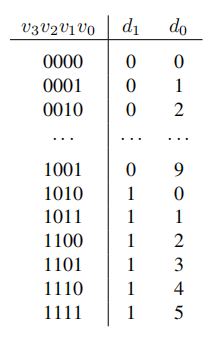
\includegraphics[width=4cm]{source/picture/Lab2/Lab2_table1.png}
                \hfill
                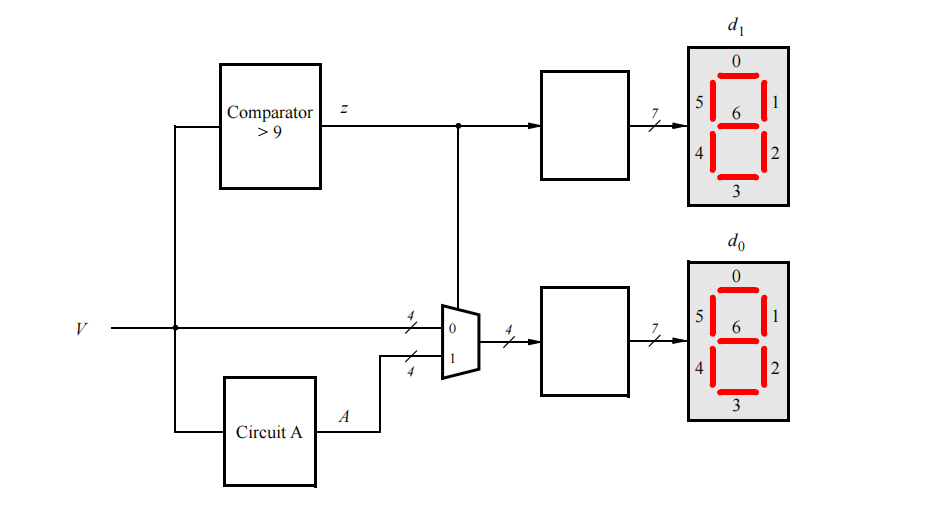
\includegraphics[width=10cm]{source/picture/Lab2/Lab2_figure1.png}
                \hfill
            \end{figure}
            \item  For the input values V ≤ 9, \textbf{the circuit A} does not matter, because the multiplexer in Figure above  just selects V in these cases. But for the input values V > 9, the multiplexer will select A.
        \end{enumerate}
    \item [] \textbf{SOLUTION}
        \begin{itemize}
            \item [] \textbf{Circuit A} is implemented using the hint of the requirement above.
                \begin{lstlisting}[language=verilog]
module circuitA(A_in, A_out);
	input		[3:0]A_in;
	output	[3:0]A_out;
	
	assign	A_out[3] = 0;
	assign 	A_out[2] = A_in[2]& A_in[1];
	assign	A_out[1] = A_in[2]&~A_in[1];
	assign 	A_out[0] = A_in[2]& A_in[0]  
					      +~A_in[2]&~A_in[0];
			
endmodule
                \end{lstlisting}
            \item [] \textbf{comparew9} indicate if the input greater than 9.
                \begin{lstlisting}[language=verilog]
module comparew9(com_in, com_out);
	input 	[3:0]com_in;
	output	com_out;
	assign 	com_out = com_in[3] & (com_in[2]|com_in[1]);
endmodule
                \end{lstlisting}
            \item [] \textbf{one\_to\_4btis} is used for translate the output of comparew9 block from 1 bits to 4 bits
                \begin{lstlisting}[language=verilog]
module multi_4bits(out, in0, in1, s);
	input		[3:0]in0,in1;
	input		s;
	output	[3:0]out;
	
	assign out = (in0&{4{~s}})|(in1&{4{s}}); 
endmodule
                \end{lstlisting}            
            \item [] \textbf{multi\_4bits} is user to choose the signal from \textbf{circuitA} and input, if input > 9, choose the result of block \textbf{circuitA.}
                \begin{lstlisting}[language=verilog]
module one_to_4bits(in,out);
	input		in;
	output	[3:0]out;
	assign 	out = (4'b0000) | in;
endmodule
                \end{lstlisting}               
            \item [] Finally, we wired these parts together. 
            \begin{figure}[h]
                \centering
                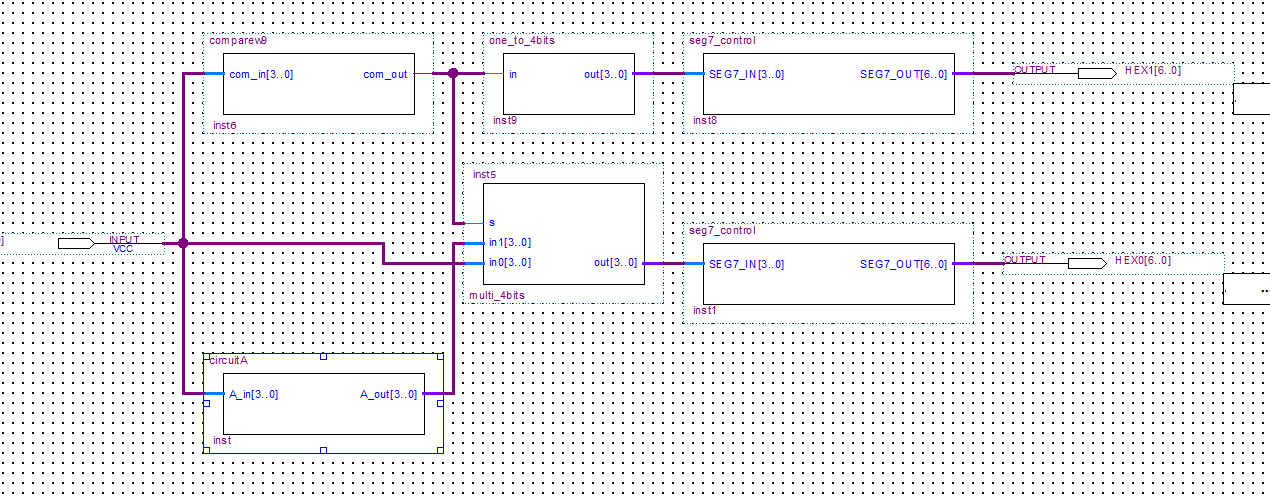
\includegraphics[width=\textwidth]{source/picture/Lab2/Lab2_2.png}
            \end{figure}
        \end{itemize}
\end{itemize}
\clearpage
\section{Part IV}
\begin{itemize}
    \item []\textbf{REQUIREMENT}
        \begin{enumerate}
            \item In part II we discussed the conversion of binary numbers into decimal digits. For this part you are to design a circuit that has two decimal digits, X and Y , as inputs. Each decimal digit is represented as a 4-bit number. In technical literature this is referred to as the binary coded decimal (BCD) representation.
            \item You are to design a circuit that adds the two BCD digits. The inputs to your circuit are the numbers X and Y , plus a carry-in, $c_{in}$. When these inputs are added, the result will be a 5-bit binary number. But this result is to be displayed on 7-segment displays as a two-digit BCD sum $S_1S_0$. 
        \end{enumerate}
    \item []\textbf{SOLUTION}
        \begin{itemize}
            \item []In this design, we use 2 block, namely: \textbf{sum4bits} and \textbf{display7SEG}.
                \begin{itemize}
                    \item []\textbf{Sum4bits} is the combination of 4 full-adder block.
                        \begin{lstlisting}[language=verilog]
module sum4bits(A,B,C_IN,SUM,C_OUT);
	input		[3:0]A,B;
	input		C_IN;
	output	[3:0]SUM;
	output	C_OUT;
	wire		C_1, C_2, C_3;
	full_adder inst1 (.a(A[0]), .b(B[0]), .c_i(C_IN),                      .s(SUM[0]), .c_o(C1));
	full_adder inst2 (.a(A[1]), .b(B[1]), .c_i(C1),                        .s(SUM[1]), .c_o(C2));
	full_adder inst3 (.a(A[2]), .b(B[2]), .c_i(C2),                        .s(SUM[2]), .c_o(C3));
	full_adder inst4 (.a(A[3]), .b(B[3]), .c_i(C3),                        .s(SUM[3]), .c_o(C_OUT));
endmodule
module full_adder(a,b,c_i,s,c_o);
	input 	a,b,c_i;
	output	s, c_o;
	assign 	s 		= c_i ^ (a^b);
	assign 	c_o	= (c_i & (a^b)) | (b & ~(a^b));
endmodule 
                        \end{lstlisting}
                    \item []\textbf{display7SEG}
                        \begin{lstlisting}[language=verilog]
module display7SEG(num, carry , hex0, hex1);
	input 	[3:0]num;
	input 	carry;
	output	[6:0]hex0, hex1;
	wire		[3:0]A_out;
	wire 		[3:0]num_plus6;
	wire		select;
	wire		com_out;
	wire		[3:0]seg7_1_in;
	wire		[3:0]seg7_0_in;
	circuitA 		inst0	(.A_in(num), .A_out(A_out));
	comparew9 		inst1	(.com_in(num),                                        .com_out(com_out));
	or select_char_1 		(select,carry,com_out);
	multi_4bits 	inst4	(.out(seg7_0_in), .in0(num),                          .in1(A_out), .s(select));
	one_to_4bits 	inst5	(.out(seg7_1_in),                                     .in(select));
	seg7_control 	inst6	(.SEG7_IN(seg7_0_in),                                 .SEG7_OUT(hex0));
	seg7_control 	inst7	(.SEG7_IN(seg7_1_in),                                 .SEG7_OUT(hex1));
endmodule
                        \end{lstlisting}
                    \item [] In \textbf{module part4}
                        \begin{lstlisting} [language=verilog]
module part4(X,Y,HEX0,HEX1);
	input 	[3:0]X,Y;
	output	[6:0]HEX0,HEX1;
	wire [3:0]num;
	wire carry;
	sum4bits 	inst0 (.A(X), .B(Y), .C_IN(0), .SUM(num), .C_OUT(carry));
	display7SEG	inst1 (.num(num), .carry(carry), .hex0(HEX0), .hex1(HEX1));
endmodule
                        \end{lstlisting}
                \end{itemize} This is our design
                    \begin{figure}[h]
                        \centering
                        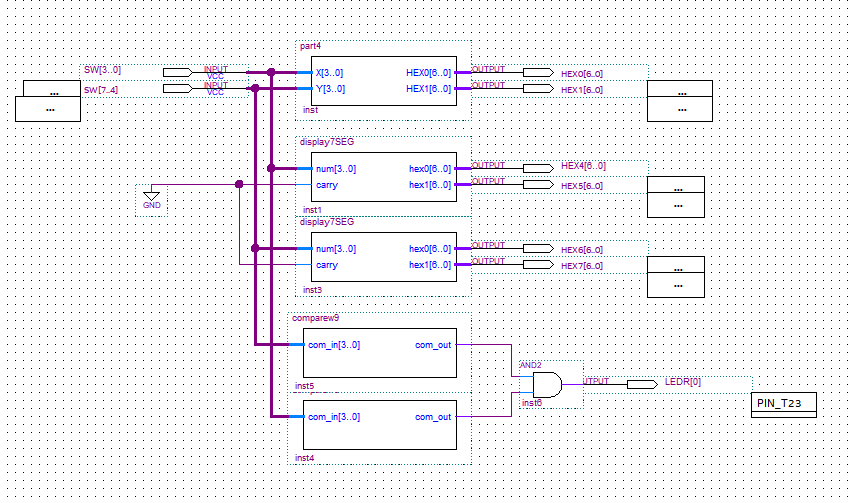
\includegraphics[width=\textwidth]{source/picture/Lab2/Lab2_4.png}
                    \end{figure}
        \end{itemize}
    
\end{itemize}
\clearpage
\chap{Latches, Flip-flops, and Registers}

\section{Part V}
\begin{itemize}
    \item []\textbf{REQUIREMENT} 
        \begin{enumerate}
            \item We wish to display the hexadecimal value of an 8-bit number A on the two 7-segment displays HEX3 - 2. We also wish to display the hex value of an 8-bit number B on the two 7-segment displays \textbf{HEX1 - 0}. 
            \item The values of A and B are inputs to the circuit which are provided by means of switches \textbf{SW7-0}. To input the values of A and B, first set the switches to the desired value of A, store these switch values in a register, and then change the switches to the desired value of B. Finally, use an adder to generate the arithmetic sum S = A + B, and display this sum on the 7-segment displays HEX5 - 4. Show the carry-out produced by the adder on LEDR[0].
        \end{enumerate}
    \item []\textbf{SOLUTION}
        \begin{itemize}
            \item []For this part, we use 2 different D\_latch with 1 Enable pin to store the input into A and B
                \begin{lstlisting}[language = verilog]
    D_latch     inst1 (.CLK(CLK),  .D(Num), .Q(A));
    D_latch     inst2 (.CLK(~CLK), .D(Num), .Q(B));
                \end{lstlisting}
            \item []Then, we use block sum8bits which is the combination of 2 sum4bits blocks we mentioned before, to do the sum between A and B.
                \begin{lstlisting}[language = verilog]
    sum8bits	sum	(.A(A), .B(B), .C_IN(0), .SUM(Sum), .C_OUT(C_out));            \end{lstlisting}
        \end{itemize}
    \item []\textbf{VERIFICATION}
        \begin{figure}[h]
            \centering
            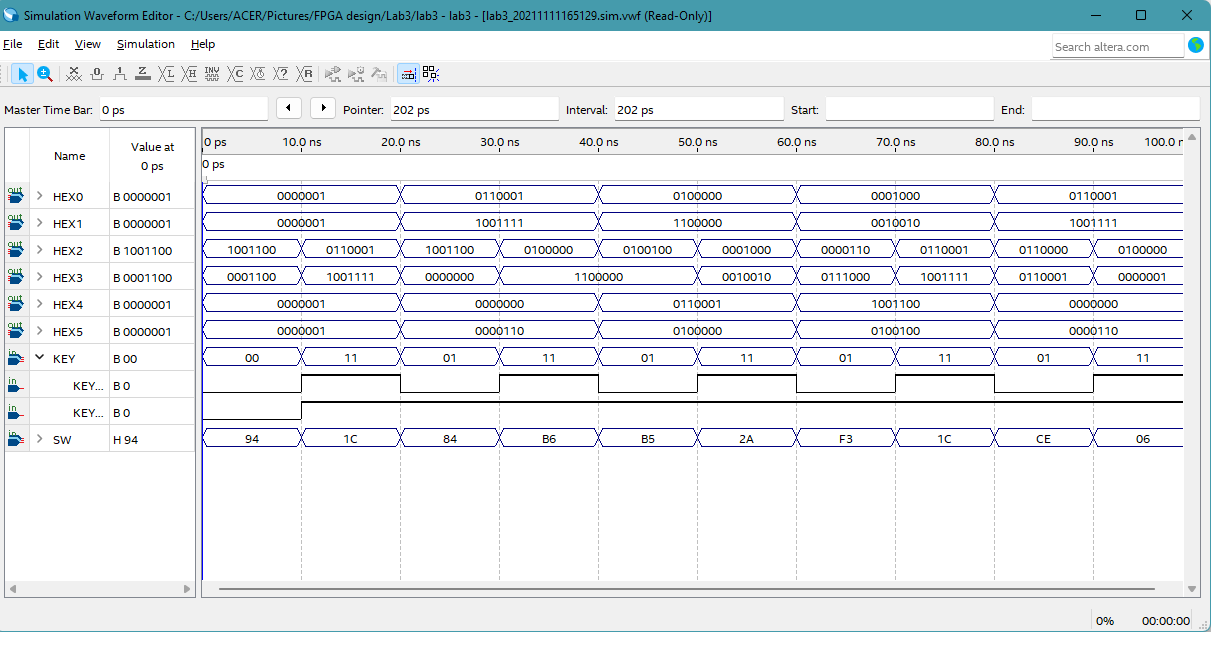
\includegraphics[scale = 0.5]{source/picture/lab3/lab3.png}
            \caption{Simulation Result}
        \end{figure}
\end{itemize}

\chap{Counters}
\section{Part V}
\begin{itemize}
    \item []\textbf{REQUIREMENT}
        \begin{enumerate}
            \item Augment your circuit from Part IV so that it can rotate the word over all of the 7-segment displays on your DE-series board. 
            \item The shifting pattern for the DE10-Lite is shown in Table below. Your can base on this table to create your own table for DE2i-150.
                \begin{figure}[h]
                    \centering
                    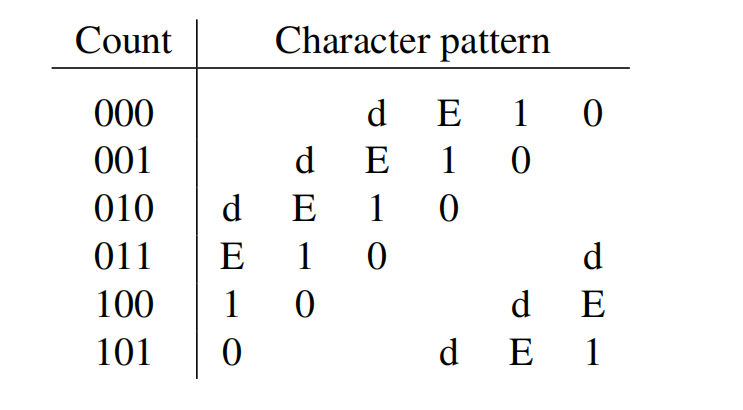
\includegraphics[width=10cm]{source/picture/lab4/Lab4_table1.png}
                    \caption{Rotating the word on six display}
                \end{figure}
        \end{enumerate}
    \item []\textbf{SOLUTION}
        \begin{itemize}
            \item []To use the clock of the board which has the frequency equal to 50MHz, we have to create the counter with in the input is the board’s clock and the output which just equal to 1 when                    
                \begin{lstlisting}[language = verilog]
always @(posedge CLK) begin
    if (Q == 50000000) flag<=1;
    else flag <= 50000000;
    
    if (!CLR | Q>50000000)  Q<= 0;
    else if (EN) Q <= Q + 1;
end

always @(posedge flag) begin
    if (!CLR | C>7)  C<= 0;
    else if (EN) C <= C + 1;
end
                    \end{lstlisting}
            \item []Each time the output of the counter equal to 1, we update the value of 8 7-segment leds by follow module.
                \begin{lstlisting}[language = verilog]
module update_display(out, val);
	input [2:0]val;
	output[55:0]out;
	
	wire [55:0]temp = 56'b111111111111111111111111111110100001000011001001001111011;
	wire [55:0]templong = temp<<(7*val);
	wire [55:0]tempshort = temp>>(56-7*val);
	
	assign out = templong | tempshort;

endmodule
                    \end{lstlisting}
            \item[]Ansd this is the entire design
                \begin{lstlisting}[language = verilog]
always @(posedge CLK) begin
    if (Q == 50000000) flag<=1;
    else flag <= 50000000;
    
    if (!CLR | Q>50000000)  Q<= 0;
    else if (EN) Q <= Q + 1;
end

always @(posedge flag) begin
    if (!CLR | C>7)  C<= 0;
    else if (EN) C <= C + 1;
end
always @(HEX_BUS) HEX = HEX_BUS;


update_display inst1(.out(HEX_BUS), .val(C[2:0]));
assign {HEX7,HEX6,HEX5,HEX4,HEX3,HEX2,HEX1,HEX0} = HEX;
                \end{lstlisting}
            \end{itemize}
    \item[]\textbf{VERIFICATION}
        \begin{figure}[h]
            \centering
            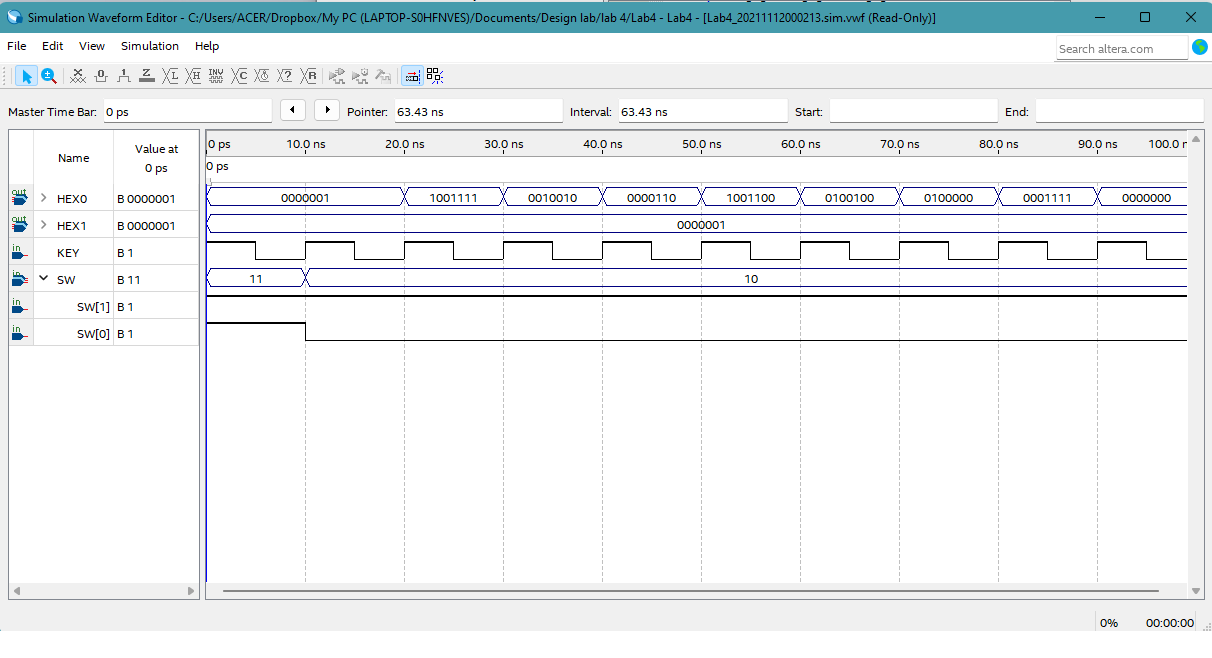
\includegraphics[scale = 0.5]{source/picture/lab4/part1.png}
            \caption{Simulation result}
        \end{figure}
\end{itemize}
\clearpage
\chap{Timers and Real-time Clock}

\section{Part IV}
An early method of telegraph communication was based on the Morse code. This code uses patterns of short and long pulses to represent a message. Each letter is represented as a sequence of dots (a short pulse), and dashes (a long pulse). For example, the first eight letters of the alphabet have the following representation:
\begin{figure}[h]
    \centering
    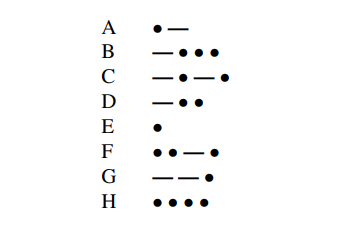
\includegraphics[scale = 0.80]{source/picture/Lab5/Lab5_1.png}
\end{figure}\\
\begin{itemize}
    \item[]\textbf{REQUIREMENT}
        \begin{enumerate}
            \item Design and implement a circuit that takes as input one of the first eight letters of the alphabet and displays the Morse code for it on a red LED.
            \item Your circuit should use switches $SW_{2-0}$ and pushbuttons $KEY_{1-0}$ as inputs. When a user presses $KEY_1$, the circuit should display the Morse code for a letter specified by $SW_{2-0}$ (000 for A, 001 for B, etc.), using 0.5-second pulses to represent dots, and 1.5-second pulses to represent dashes.
            \item Pushbutton $KEY_0$ should function as an asynchronous reset. A high-level schematic diagram of the circuit is shown in Figure 2.
                \begin{figure}[h]
                    \centering
                    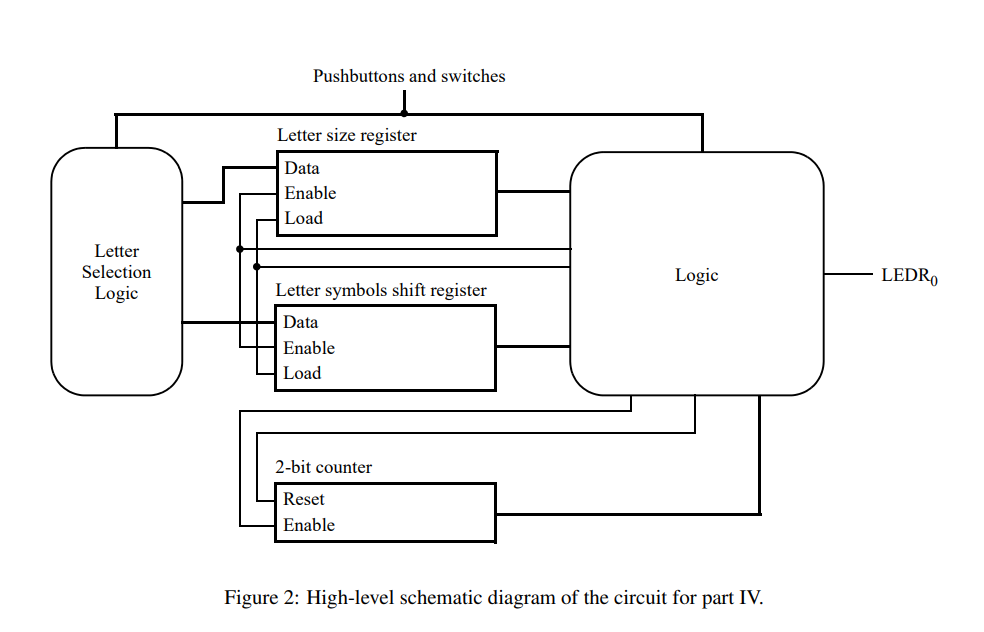
\includegraphics[scale = 0.50]{source/picture/Lab5/Lab5_2.png}
                \end{figure}
        \end{enumerate}
\clearpage
    \item[]\textbf{SOLUTION}
        \begin{itemize}
            \item [] We base on the hint given; we translate the input which has a 3-bit length into the signal 13 bits.
                \begin{lstlisting}[language = verilog]
module translate_signal(in, out);
	input		[3:0]in;
	output	reg [12:0]out;
	
	always begin
		if (in==0) out=13'b0000000111010;
		if (in==1) out=13'b0001010101110;
		if (in==2) out=13'b0101110101110;
		if (in==3) out=13'b0000010101110;
		if (in==5) out=13'b0001011101010;
		if (in==4) out=13'b0000000000010;
		if (in==6) out=13'b0001110111010;
		if (in==7) out=13'b0000010101010;
	end
endmodul
                \end{lstlisting}
            \item [] After translating, we shift left 13 times, each time, if that bit is 1 we turn on the led, if that  bit is equal to 0, we turn off the led. The period for each clock is 0.5 seconds.
                \begin{lstlisting}[language=verilog]
module part4 (CLK, RESET, EN, code, led);
	input		CLK, RESET, EN;
	input		[2:0]code;
	output	led;

	reg 		[2:0]numb;
	wire		[12:0]decode	 /*synthesis keep*/;
	wire		time_start		 /*synthesis keep*/;
	
	
	
	counter 		sub_clk 	(.CLK(CLK), .RESET(RESET), .K(25000000), .rollover(time_start), .Q());
	translate_signal	inst0 	(.in(code), .out(decode));
	defparam sub_clk.n = 25;
	
	always @(posedge time_start) numb<=numb+1;
	assign led = decode[numb] & EN;
	
				
endmodule
                \end{lstlisting}
        \end{itemize}
\end{itemize}

\clearpage

\chap{ Adders, Subtractors, and Multipliers}

\section{Introduction}
The purpose of this exercise is to examine arithmetic circuits that add, subtract, and multiply numbers. Each circuit will be described in Verilog and implemented on an Intel FPGA DE10-Lite, DE0-CV, DE1-SoC, or DE2- 115 board.
\section{Part IV}
\begin{itemize}
    \item [] \textbf{REQUIREMENT}
        \begin{enumerate}
            \item In Part III, an array multiplier was implemented using full adder modules. At a higher level, a row of full adders functions as an n-bit adder and the array multiplier circuit can be represented as shown in Figure 5.
                 \begin{figure}[h]
                    \centering
                    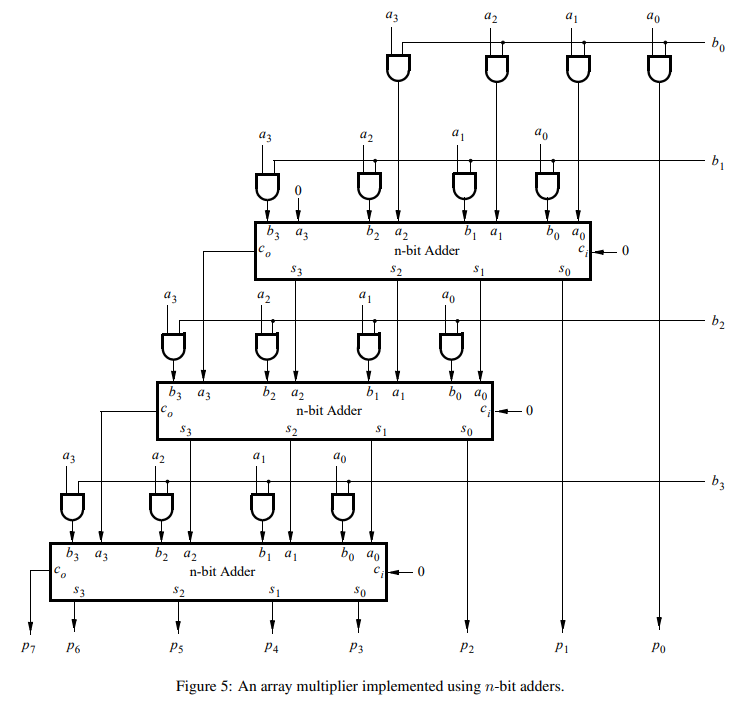
\includegraphics[scale = 0.75]{source/picture/Lab6/Lab6_4_0.png}
                \end{figure}
\clearpage
            \item Each n-bit adder adds a shifted version of A for a given row and the partial product of the row above. Abstracting the multiplier circuit as a sequence of additions allows us to build larger multipliers. The multiplier should consist of n-bit adders arranged in a structure shown in Figure 5. Use this approach to implement an 8 x 8 multiplier circuit with registered inputs and outputs, as shown in Figure 6.
                \begin{figure}[h]
                    \centering
                    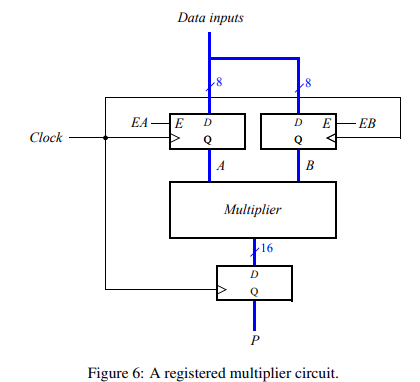
\includegraphics[scale = 0.9]{source/picture/Lab6/Lab6_4_1.png}
                \end{figure}
        \end{enumerate}
    \item [] \textbf{SOLUTION}
        \begin{lstlisting}[language=verilog]
module part4(CLK, IN,EA,EB,P);
	input		CLK, EA, EB;
	input		[7:0]IN;
	output	[15:0]P;
	
	wire	[7:0] A,B;
	wire	[15:0]SUM;
	wire	[7:0] adder1_in0, adder1_in1;
	wire	[7:0] adder2_in0, adder2_in1;
	wire 	[7:0] adder3_in0, adder3_in1;
	wire	[7:0] adder4_in0, adder4_in1;
	wire	[7:0] adder5_in0, adder5_in1;
	wire 	[7:0] adder6_in0, adder6_in1;
	wire	[7:0] adder7_in0, adder7_in1;

	D_FF	inputa_ff (.CLK(CLK), .EN(EA), .D(IN),  .Q(A));
	D_FF	inputb_ff (.CLK(CLK), .EN(EB), .D(IN),  .Q(B));
	D_FF	output_ff (.CLK(CLK), .EN(1),  .D(SUM), .Q(P));
	
	multiply_Nx1	inst0		(.A(A), .B(B[0]),      .P({adder1_in0[6:0],SUM[0]}));
	multiply_Nx1	inst1		(.A(A), .B(B[1]), .P(adder1_in1));
	multiply_Nx1	inst2		(.A(A), .B(B[2]), .P(adder2_in1));
	multiply_Nx1	inst3		(.A(A), .B(B[3]), .P(adder3_in1));
	multiply_Nx1	inst4		(.A(A), .B(B[4]), .P(adder4_in1));
	multiply_Nx1	inst5		(.A(A), .B(B[5]), .P(adder5_in1));
	multiply_Nx1	inst6		(.A(A), .B(B[6]), .P(adder6_in1));
	multiply_Nx1	inst7		(.A(A), .B(B[7]), .P(adder7_in1));
	
	sumNbits adder1 (.A(adder1_in0), .B(adder1_in1), .C_IN(0) ,.SUM({adder2_in0[2:0],SUM[1]}) ,.C_OUT(adder2_in0[3]));
	sumNbits adder2 (.A(adder2_in0), .B(adder2_in1), .C_IN(0) ,.SUM({adder3_in0[2:0],SUM[2]}) ,.C_OUT(adder3_in0[3]));
	sumNbits adder3 (.A(adder3_in0), .B(adder3_in1), .C_IN(0) ,.SUM({adder4_in0[2:0],SUM[3]}) ,.C_OUT(adder4_in0[3]));
	sumNbits adder4 (.A(adder4_in0), .B(adder4_in1), .C_IN(0) ,.SUM({adder5_in0[2:0],SUM[4]}) ,.C_OUT(adder5_in0[3]));
	sumNbits adder5 (.A(adder5_in0), .B(adder5_in1), .C_IN(0) ,.SUM({adder6_in0[2:0],SUM[5]}) ,.C_OUT(adder6_in0[3]));
	sumNbits adder6 (.A(adder6_in0), .B(adder6_in1), .C_IN(0) ,.SUM({adder7_in0[2:0],SUM[6]}) ,.C_OUT(adder7_in0[3]));
	sumNbits adder7 (.A(adder7_in0), .B(adder7_in1), .C_IN(0) ,.SUM(SUM[14:7]) 		  ,.C_OUT(SUM[15]));
	
	defparam inputa_ff.n_bits = 8;
	defparam inputb_ff.n_bits = 8;
	defparam output_ff.n_bits = 16;
	
	defparam inst0.n_bits = 8;
	defparam inst1.n_bits = 8;
	defparam inst2.n_bits = 8;
	defparam inst3.n_bits = 8;
	defparam inst4.n_bits = 8;
	defparam inst5.n_bits = 8;
	defparam inst6.n_bits = 8;
	defparam inst7.n_bits = 8;
	
	defparam	adder1.n_bits = 8;
	defparam	adder2.n_bits = 8;
	defparam	adder3.n_bits = 8;
	defparam	adder4.n_bits = 8;
	defparam	adder5.n_bits = 8;
	defparam	adder6.n_bits = 8;
	defparam	adder7.n_bits = 8;
endmodule
        \end{lstlisting}
   \item[]\textbf{VERIFICATION}
        \begin{figure}[h]
            \centering
            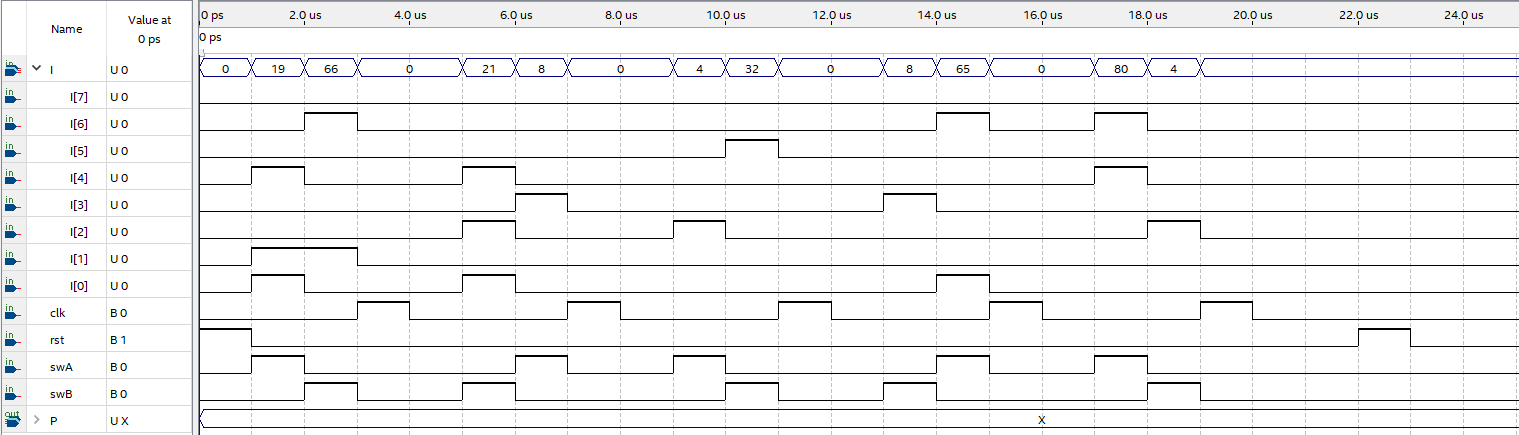
\includegraphics[width=\textwidth]{source/picture/Lab6/Lab6 _4.png}
            \caption{Simulation Result}
        \end{figure}
\end{itemize}
\clearpage
\section{Part 5}
\begin{itemize}
    \item []\textbf{REQUIREMENT}
        \begin{enumerate}
            \item Part IV showed how to implement multiplication A × B as a sequence of additions, by accumulating the shiftedversions of A one row at a time. Another way to implement this circuit is to perform addition using an adder tree. An adder tree is a method of adding several numbers together in a parallel fashion.
                \begin{figure}[h]
                    \centering
                    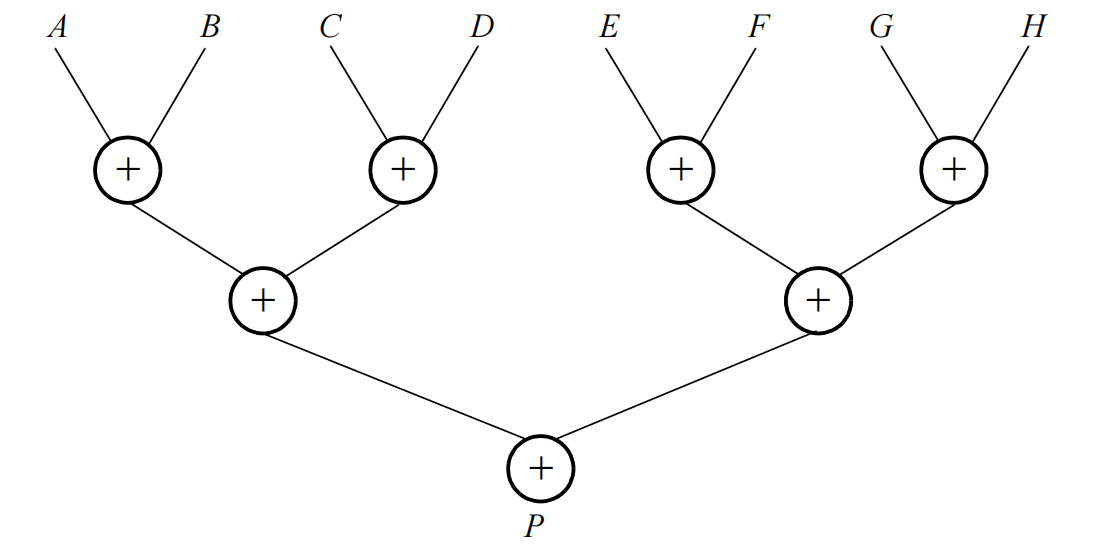
\includegraphics[width=\textwidth]{source/picture/Lab6/lab6_adder_treee.png}
                    \caption{Adder tree}
                \end{figure}
            \item In this part you are to implement an 8 x 8 multiplier circuit by using the adder-tree approach. Inputs A and B, as well as the output P should be registered as in Part IV
        \end{enumerate}
    \item []\textbf{SOLUTION}
        \begin{itemize}
            \item []In this part we try to implement multiplication by adder tree or we will add in parallel rather than sequence additions
            \item []So firstly I create \textbf{add\_8bit} module with use to calculate the sum of two numbers 8 bit.
                \begin{figure}[h]
                    \centering
                    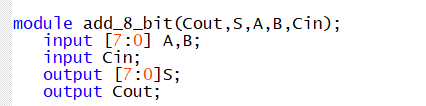
\includegraphics[width=\textwidth]{source/picture/Lab6/Lab6_add8bit.png}
                    \caption{Module add\_8\_bits}
                \end{figure}
            \item []Then create \textbf{MUL} module but now use parallel adding or (adder tree) so with A, B 8 bits number I will separate it into 8 layers and extern each layer to 8 bit.
                \begin{figure}[h]
                    \centering
                    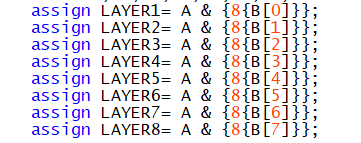
\includegraphics[width=\textwidth]{source/picture/Lab6/Lab6_mul.png}
                    \caption{Module MUL}
                \end{figure}
            \item []After having separated layers represent A,B,C … in picture then I do add operations like the image above.
                \begin{figure}[h]
                    \centering
                    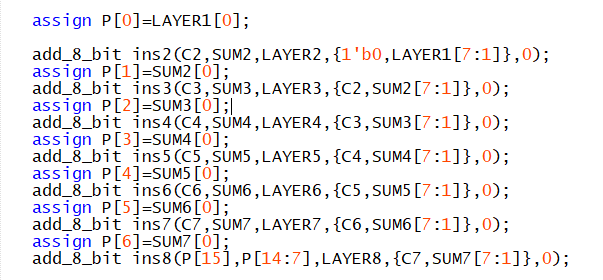
\includegraphics[width=\textwidth]{source/picture/Lab6/Lab6_rest.png}
                    \caption{Main program}

                \end{figure}
        \end{itemize}   
\end{itemize}
\clearpage

\chap{ Finite State Machines}
\section{Part II}
\begin{itemize}
    \item []\textbf{REQUIREMENT}
        \begin{enumerate}
            \item We wish to implement a finite state machine (FSM) that recognizes two specific sequences of applied input symbols, namely four consecutive 1s or four consecutive 0s. There is an input w and an output z. Whenever w = 1 or w = 0 for four consecutive clock pulses the value of z has to be 1; otherwise, z = 0. Overlapping sequences are allowed, so that if w = 1 for five consecutive clock pulses the output z will be equal to 1 after the fourth and fifth pulses.
            \item A state diagram for this FSM is shown in Figure 2. 
                \begin{figure}[h]
                    \centering
                    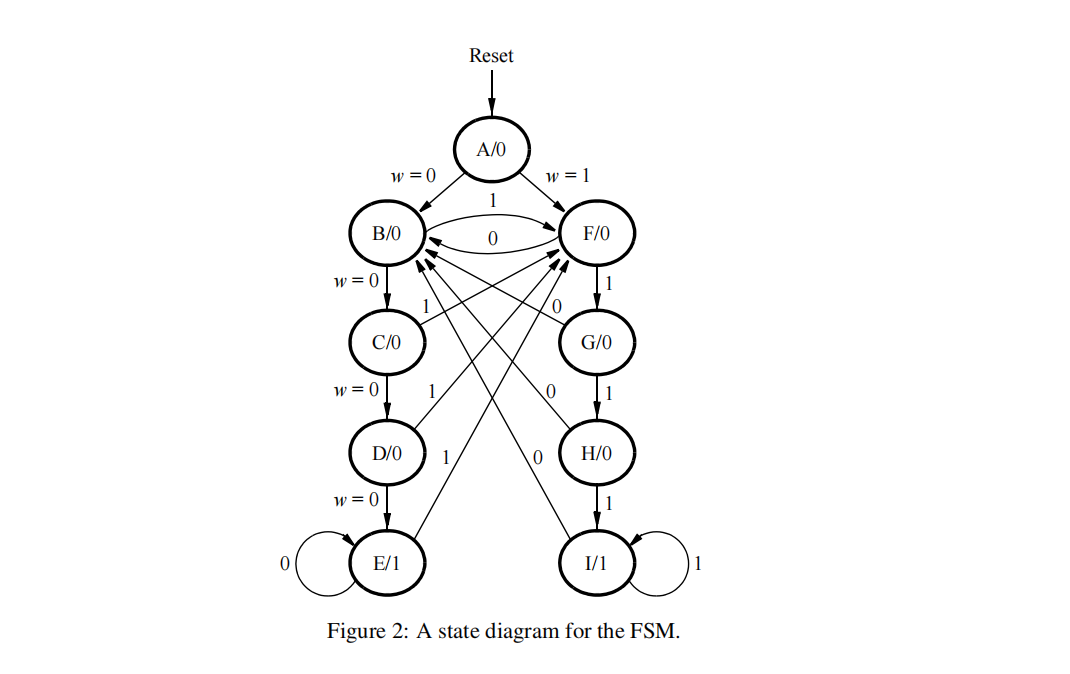
\includegraphics[scale = 0.45]{source/picture/Lab7/minh_hoa_2.png}
                \end{figure}
            \item To implement the FSM use nine state flip-flops called y8, . . . , y0 and the one-hot state assignment given in Table 1.
                \begin{figure}[h]
                    \centering
                    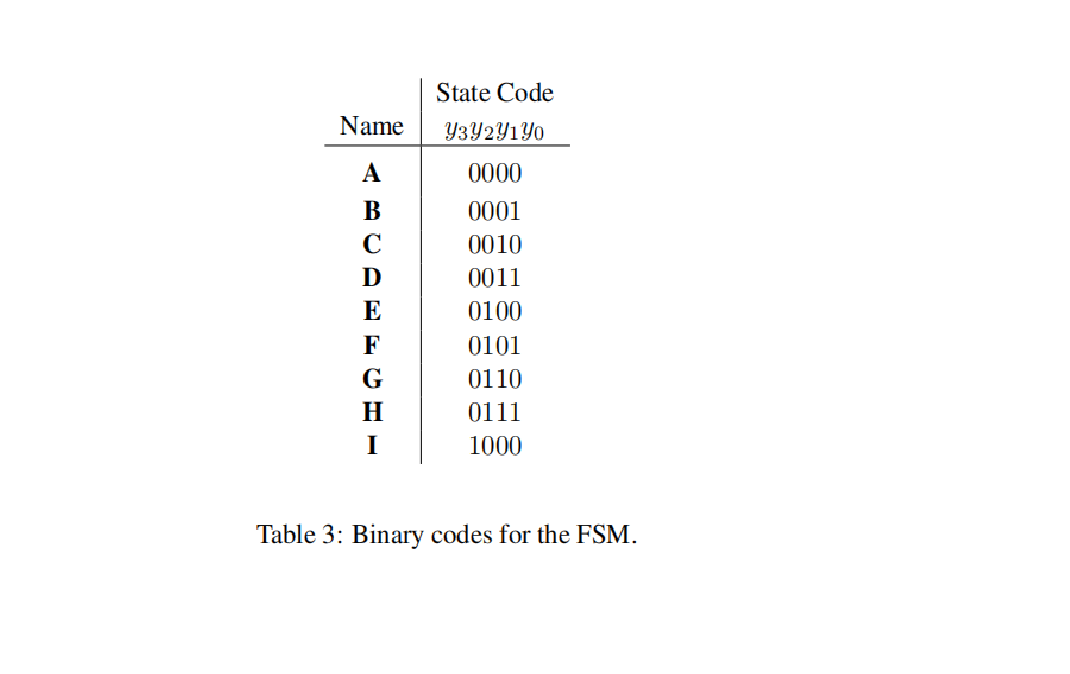
\includegraphics[scale = 0.45]{source/picture/Lab7/minh_hoa_3.png}
                \end{figure}
        \end{enumerate}
\clearpage
    \item []\textbf{SOLUTION}
        \begin{lstlisting}[language=Verilog]
module part2(CLK, RESET, IN, OUT, STATE);
	input		CLK, RESET, IN;
	output	OUT;
	output	[8:0]STATE;
	
	reg		[3:0]YQ, YD;
	parameter 	A = 4'b0000, 
                B = 4'b0001, 
                C = 4'b0010, 
                D = 4'b0011, 
                E = 4'b0100, 
                F = 4'b0101, 
                G = 4'b0110, 
                H = 4'b0111, 
                I = 4'b1000;
	
	always @(IN, YQ) begin
		case (YQ)
			A: begin if (IN) YD = F; else YD = B; end
			B: begin if (IN) YD = F; else YD = C; end
			C: begin if (IN) YD = F; else YD = D; end
			D: begin if (IN) YD = F; else YD = E; end
			E: begin if (IN) YD = F; else YD = E; end
			F: begin if (IN) YD = G; else YD = B; end
			G: begin if (IN) YD = H; else YD = B; end
			H: begin if (IN) YD = I; else YD = B; end
			I: begin if (IN) YD = I; else YD = B; end
			default: YD = 4'bxxxx;
		endcase
	end
	
	always @(posedge CLK) begin
		if (RESET) YQ<=YD;
		else YQ<=A;
	end
	
	change_signal inst0 (.in(YQ), .out(STATE));
	assign OUT = (YQ==E) | (YQ==I);
	
endmodule
        \end{lstlisting}
\clearpage
    \item []\textbf{VERIFICATION}
        \begin{figure}[h]
            \centering
            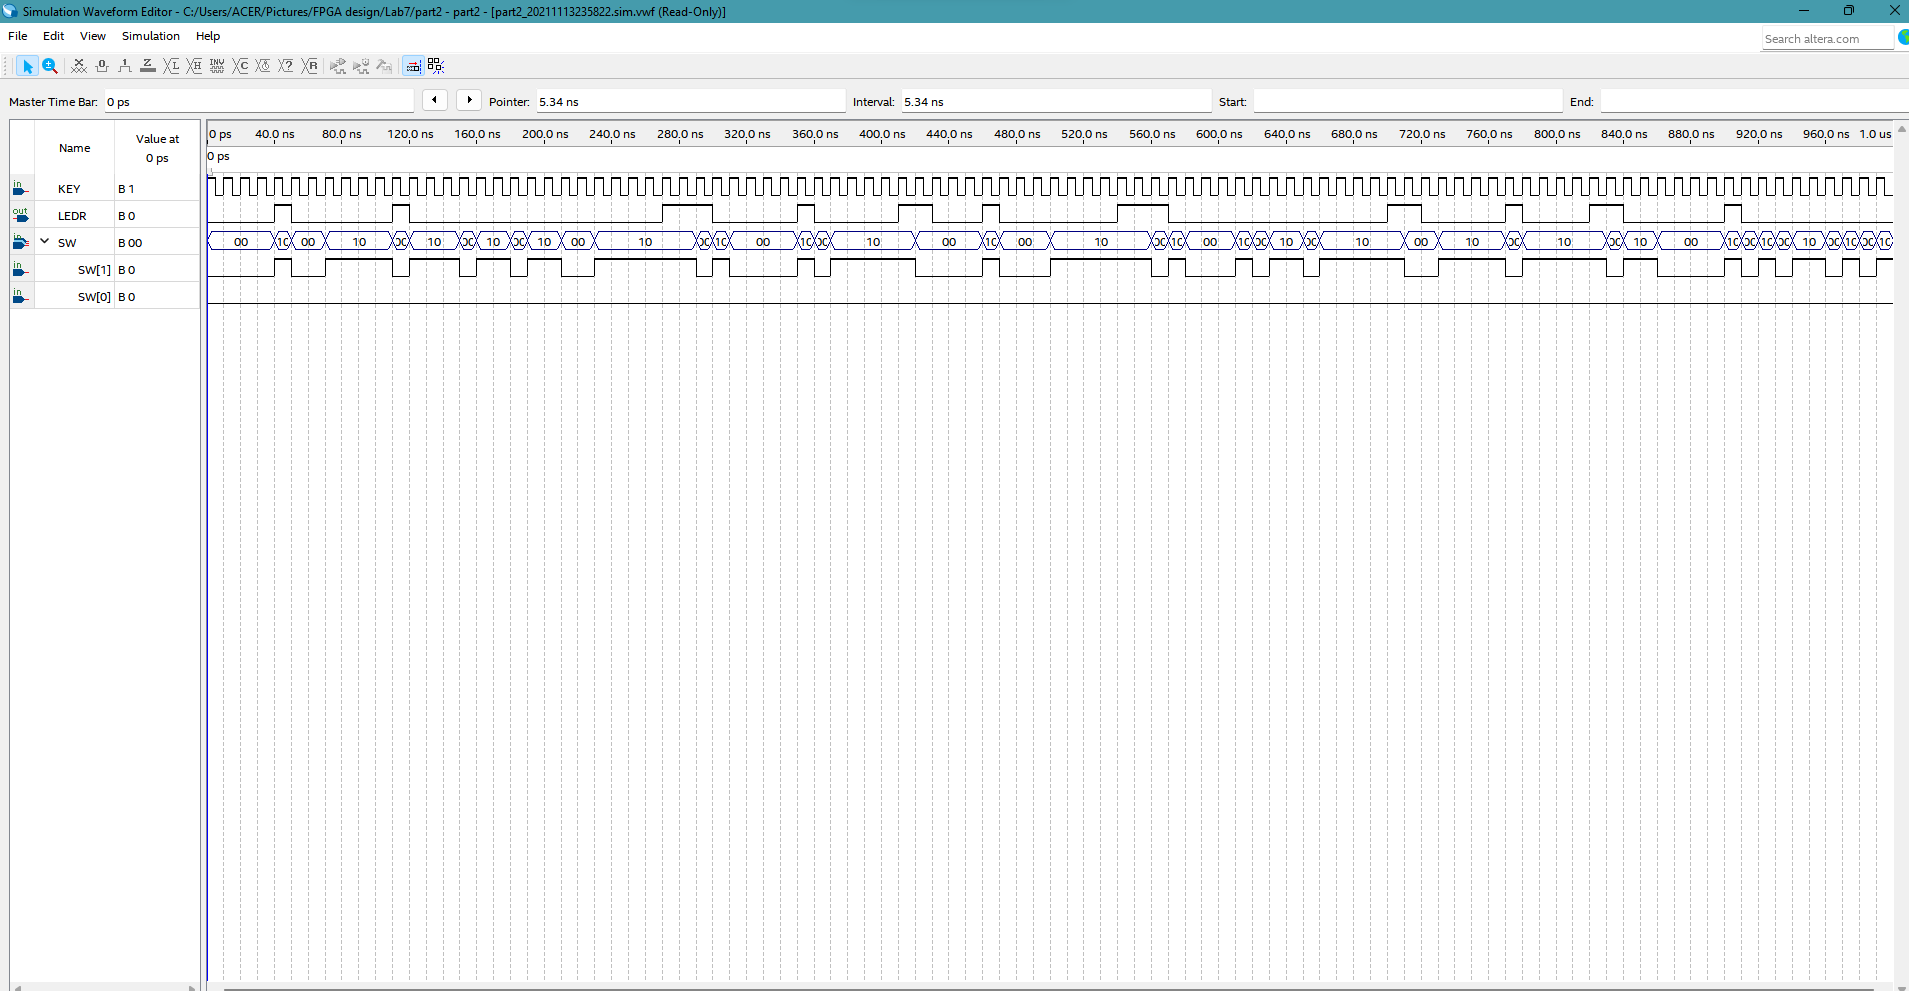
\includegraphics[scale = 0.3]{source/picture/Lab7/bai7_1.png}
            \caption{Simulation Result}
        \end{figure}
\end{itemize}
\newpage



\section{Part IV}
\begin{itemize}
    \item []\textbf{REQUIREMENT}
        \begin{enumerate}
            \item In this part of the exercise you are to implement a Morse-code encoder using an FSM. The Morse code uses patterns of short and long pulses to represent a message. Each letter is represented as a sequence of dots (a short pulse), and dashes (a long pulse). For example, the first eight letters of the alphabet have the following representation:
                \begin{figure}[h]
                    \centering
                    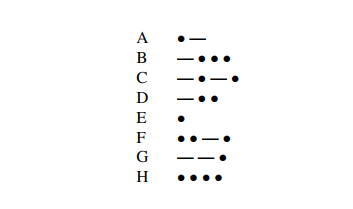
\includegraphics[scale = 0.8]{source/picture/Lab7/Lab7_1.png}
                    \caption{}
                \end{figure}
            \item Design and implement a Morse-code encoder circuit using an FSM. Your circuit should take as input one of the first eight letters of the alphabet and display the Morse code for it on a red LED. Use switches $SW_{2-0}$ and pushbuttons $KEY_{1-0}$ as inputs. When a user presses $KEY_1$, the circuit should display the Morse code for a letter specified by $SW_{2-0}$ (000 for A, 001 for B, etc.), using 0.5-second pulses to represent dots, and 1.5-second pulses to represent dashes. Pushbutton $KEY_0$ should function as an asynchronous reset. 
                \begin{figure}[h]
                    \centering
                    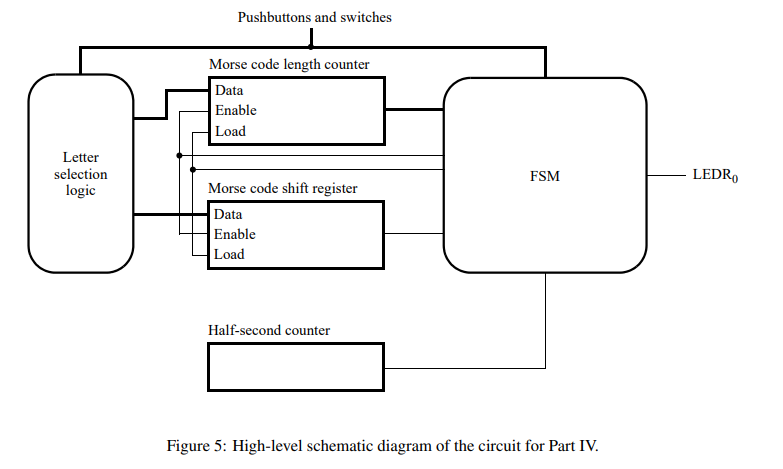
\includegraphics[scale = 0.8]{source/picture/Lab7/Lab7_2.png}
                \end{figure}
        \end{enumerate}
\clearpage

    \item []\textbf{SOLUTION}
        \begin{itemize}
            \item []Our idea is the same with the LAB5\_PART\_IV but now I try to use a state machine so firstly I create state.
                \begin{lstlisting}[language=verilog]
parameter   A=3'b000,
        B=3'b001,
        C=3'b010,
        D=3'b011,
        E=3'b100,
        F=3'b101,
        G=4'b110,
        H=3'b111;
                \end{lstlisting}
            \item []Whenever user change the input I will update the status of the machine
                \begin{lstlisting}[language=verilog]
always@(SW)
begin 
    case(SW)
        A: Y_D=A;
        B: Y_D=B;
        C: Y_D=C;
        D: Y_D=D;
        E: Y_D=E;
        F: Y_D=E;
        G: Y_D=G;
        H: Y_D=H;
    endcase
end
                \end{lstlisting}
            \item []Then when they press button Key\_1 I will update the OUTPUT\_SIGNAL
                \begin{lstlisting}[language=verilog]
always@(posedge KEY[1]) begin
        y_Q = Y_D;
        case (y_Q)
        0: SIGNAL = 14'b00101110000000; // A
        1: SIGNAL = 14'b00111010101000; // B
        2: SIGNAL = 14'b00111010111010; // C
        3: SIGNAL = 14'b00111010100000; // D
        4: SIGNAL = 14'b00100000000000; // E
        5: SIGNAL = 14'b00101011101000; // F
        6: SIGNAL = 14'b00111011101000; // G
        7: SIGNAL = 14'b00101010100000; // H
        default : SIGNAL=14'bxxxxxxxxxxxx;
        endcase
end
                \end{lstlisting}
            \item []The value of Signal have meaning that because I use a counter to count half a second and I will to change the value of LED following the index of SIGNAL ("-"=3'b111=1.5 second, "."=1b'1=0.5 second)
                \begin{lstlisting}[language=verilog]
counter_k_bit ins1(HALFSEC,Clk,KEY[0]);
defparam ins1.n=26;
defparam ins1.k=25000000;//25000000

always @(negedge Clk) begin
    if(HALFSEC==24999999) half=1;//24999999
    else half=0;
end

assign reset=KEY[1] && KEY[0];

counter_k_bit ins2(INDEX,half,reset);
defparam  ins2.n=4;
defparam  ins2.k=14;

always begin
   case (INDEX)
          0:LEDR = SIGNAL[13];
          1:LEDR= SIGNAL[12];
          2:LEDR= SIGNAL[11];
          3:LEDR= SIGNAL[10];
          4:LEDR= SIGNAL[9];
          5:LEDR= SIGNAL[8];
          6:LEDR= SIGNAL[7];
          7:LEDR= SIGNAL[6];
          8:LEDR= SIGNAL[5];
          9:LEDR= SIGNAL[4];
          10:LEDR= SIGNAL[3];
          11:LEDR= SIGNAL[2];
          12:LEDR= SIGNAL[1];
          13:LEDR= SIGNAL[0];
    endcase
end
                \end{lstlisting}
        \end{itemize}
    \item []\textbf{VERIFICATION}
        \begin{figure}[h]
            \centering
            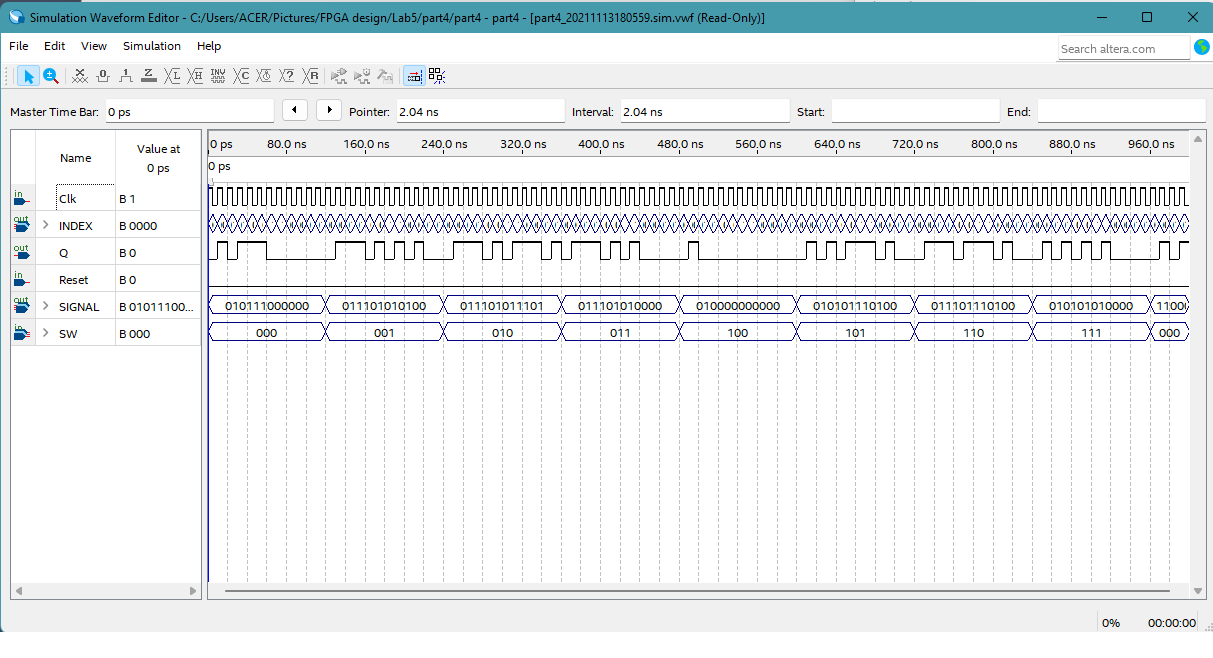
\includegraphics[scale = 0.5]{source/picture/Lab7/bai7.png}
            \caption{Simulation result}
        \end{figure}
\end{itemize}

\clearpage
\chap{ Memory Blocks}





\section{Part IV} 
The SRAM block in Figure 1 has a single port that provides the address for both read and write operations. For this part you will create a different type of memory module, in which there is one port for supplying the address for a read operation, and a separate port that gives the address for a write operation. Perform the following steps. \\
\\
    1. Create a new Quartus project for your circuit. To generate the desired memory module open the IP Catalog
and select the RAM: 2-PORT module in the Basic Functions > On Chip Memory category. As shown in
Figure 5, choose With one read port and one write port in the category called How will you be using
the dual port ram?\\
\\
Configure the memory size, clocking method, and registered ports the same way as Part II. As shown in
Figure 6 select I do not care (The outputs will be undefined) for Mixed Port Read-During-Write for
Single Input Clock RAM. This setting specifies that it does not matter whether the memory outputs the
new data being written, or the old data previously stored, in the case that the write and read addresses are
the same during a write operation.
\begin{figure}[h]
    \centering
    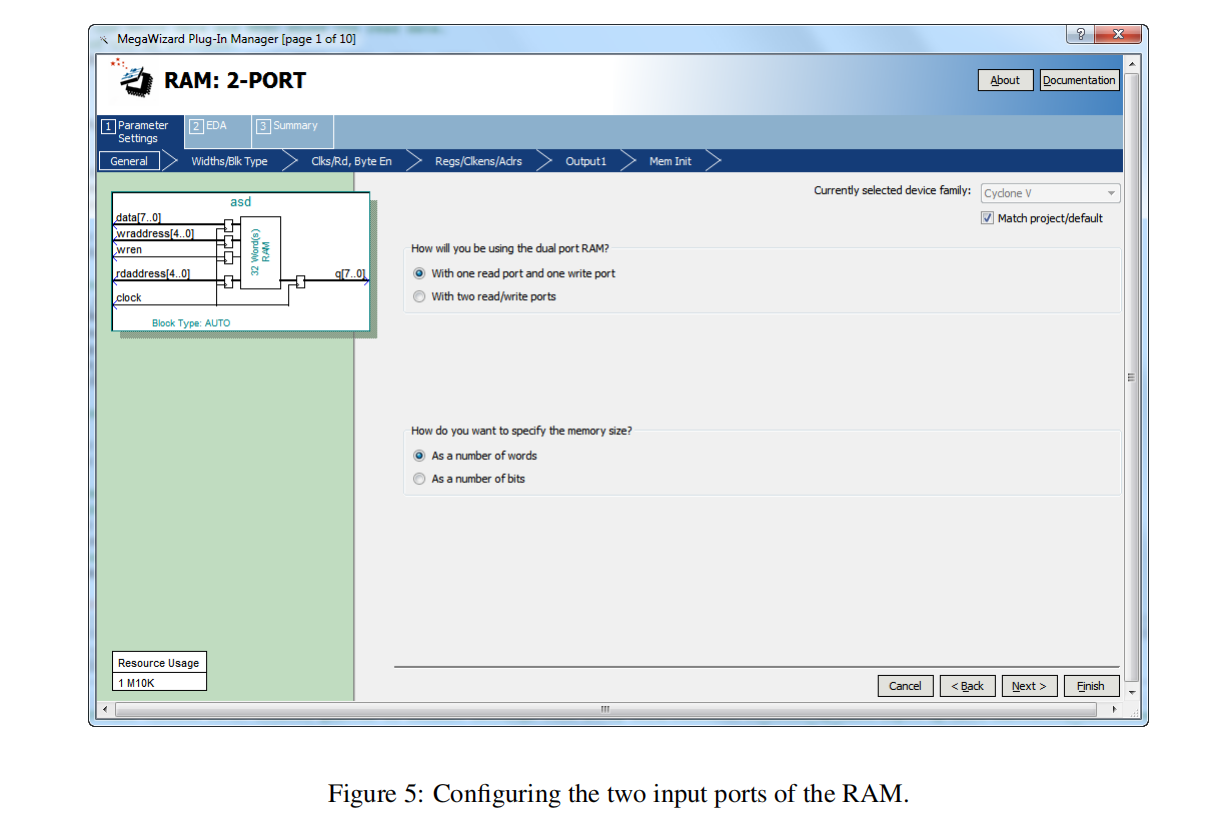
\includegraphics[scale = 0.4]{source/picture/Lab8/bai8_minhhoa1.png}
\end{figure}
\newpage

\begin{figure}[h]
    \centering
    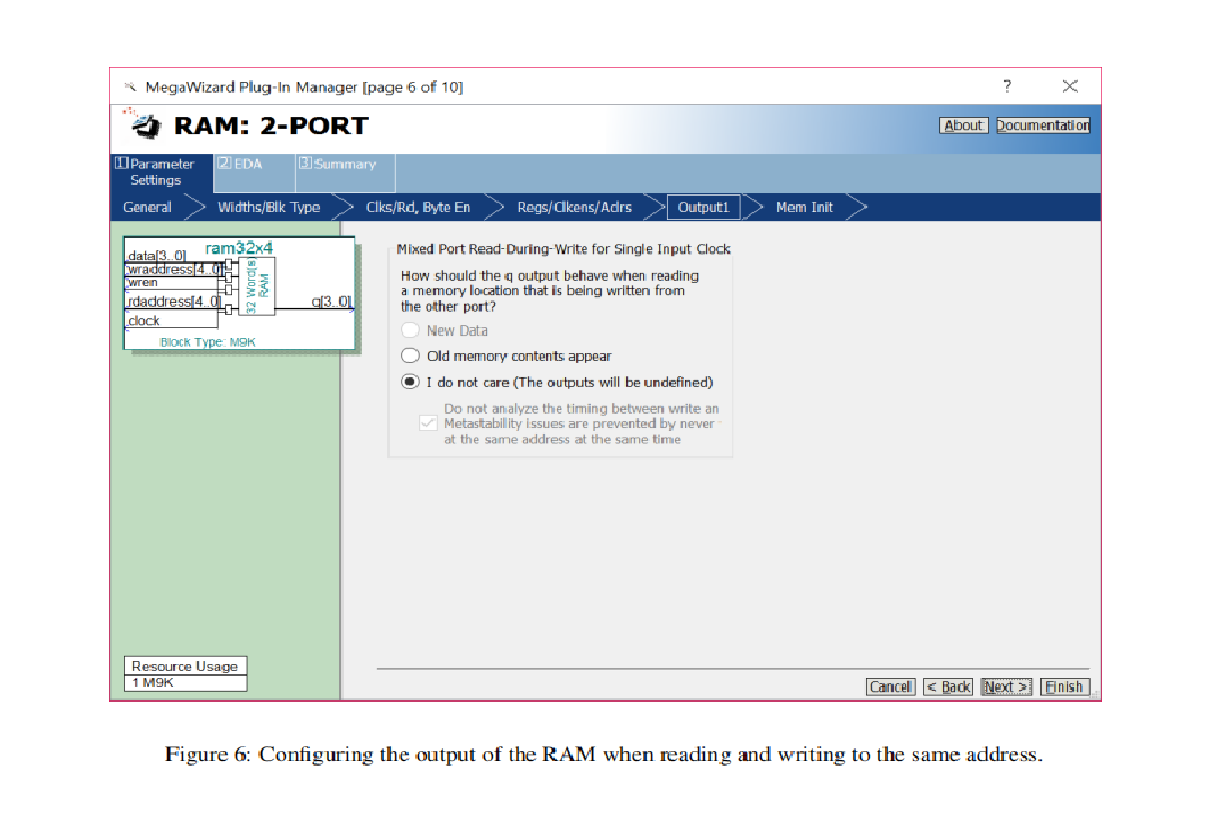
\includegraphics[scale = 0.4]{source/picture/Lab8/bai8_minhhoa2.png}
\end{figure}
Figure 7 shows how the memory words can be initialized to specific values. It makes use of a feature that
allows the memory module to be loaded with data when the circuit is programmed into the FPGA chip.
As shown in the figure, choose the setting Yes, use this file for the memory content data, and specify
the filename ram32x4.mif. An example of a MIF file is provided in Figure 8. You can also learn about the
format of a memory initialization file (MIF) by using the Quartus Help. You will need to create a MIF file
like the one in Figure 8 to test your circuit. Finish the Wizard and then examine the generated memory
module in the file ram32x4.v.

\begin{figure}[h]
    \centering
    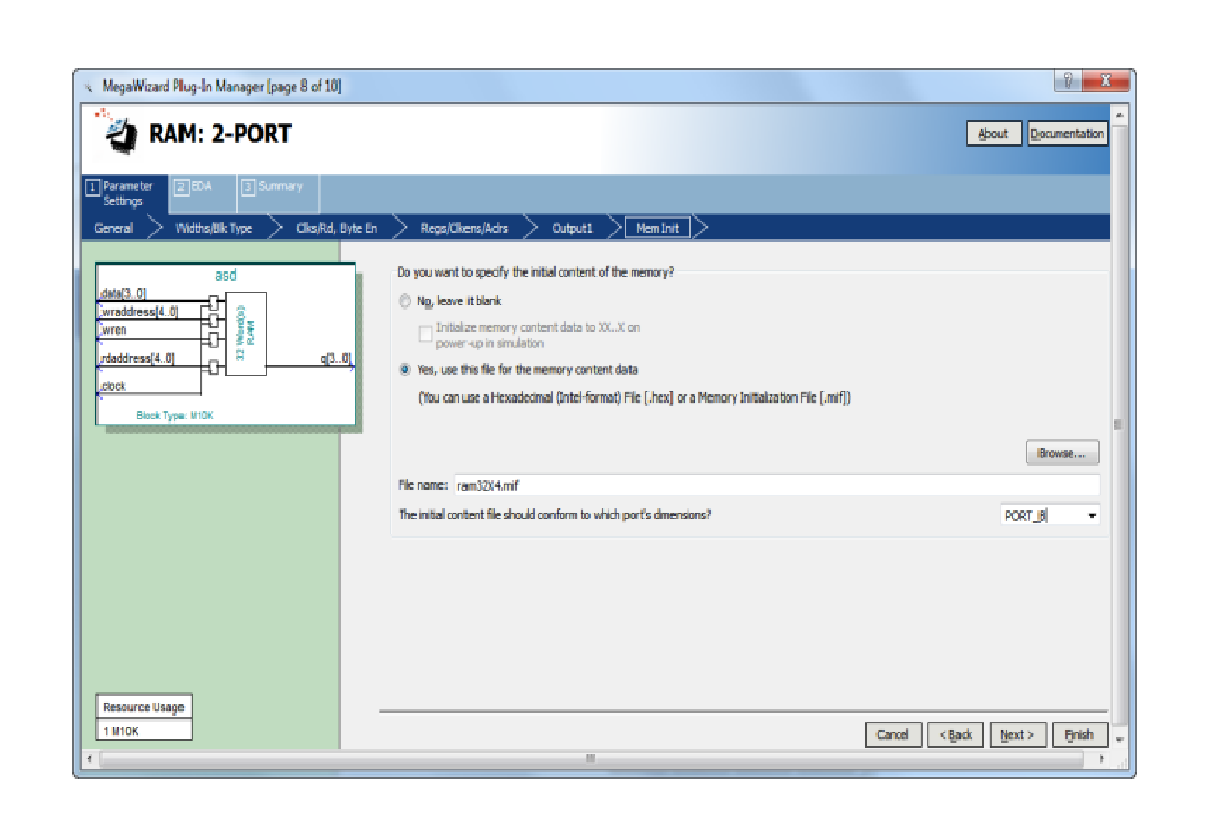
\includegraphics[scale = 0.4]{source/picture/Lab8/bai8_minhhoa3.png}
\end{figure}
\newpage
\begin{figure}[h]
    \centering
    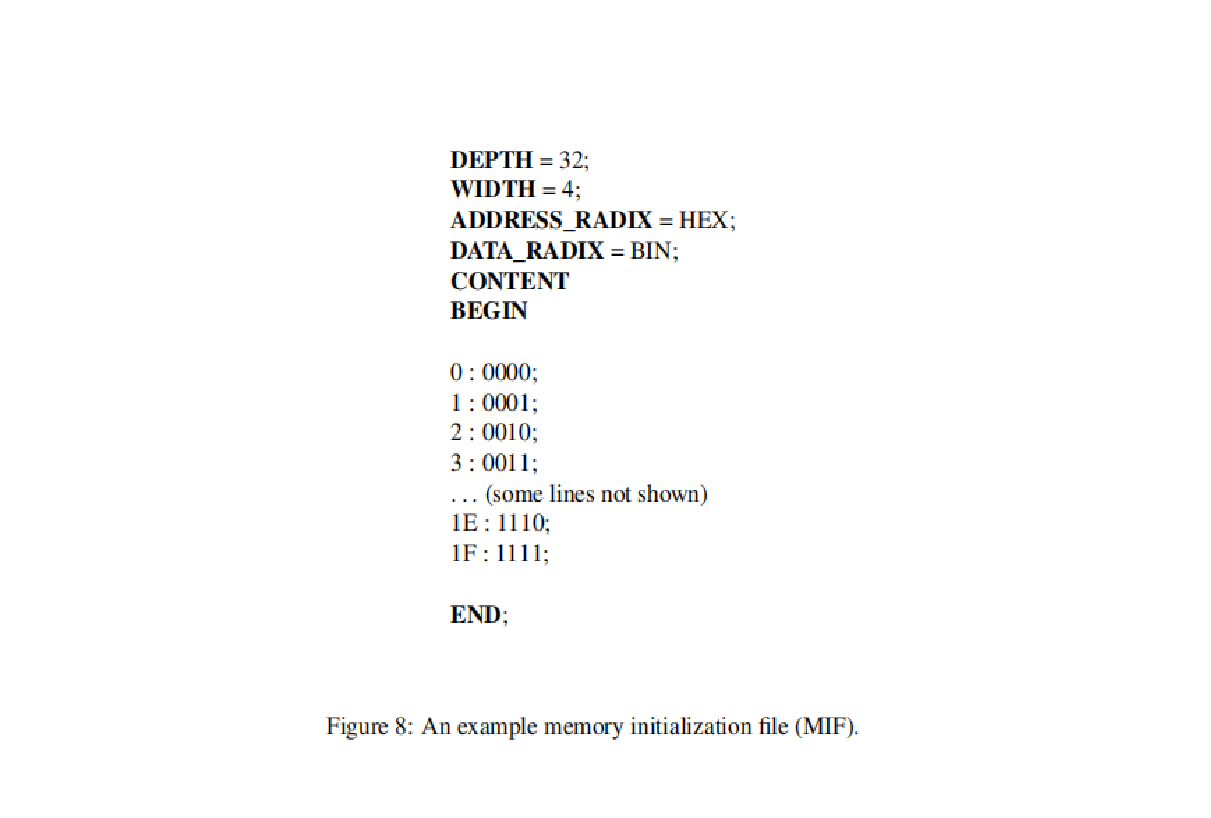
\includegraphics[scale = 0.5]{source/picture/Lab8/bai8_minhhoa4.png}
\end{figure}
2. Write a Verilog file that instantiates your dual-port memory. To see the RAM contents, add to your design a capability to display the content of each four-bit word (in hexadecimal format) on the 7-segment display 6-HEX0. Use a counter as a read address, and scroll through the memory locations by displaying each word for about one second. As each word is being displayed, show its address (in hex format) on the 7-segment displays HEX3-2. Use the 50 MHz clock, CLOCK50, and use KEY0 as a reset input. For the write address and corresponding data use switches SW8-4 and SW3-0. Show the write address on HEX5-4 and show the write data on HEX1. Make sure that you properly synchronize the slide switch inputs to the 50 MHz clock signal.\\
\\
3. Test your circuit and verify that the initial contents of the memory match your ram32x4.mif file. Make sure
that you can independently write data to any address by using the slide switches.\\

\begin{figure}[h]
    \centering
    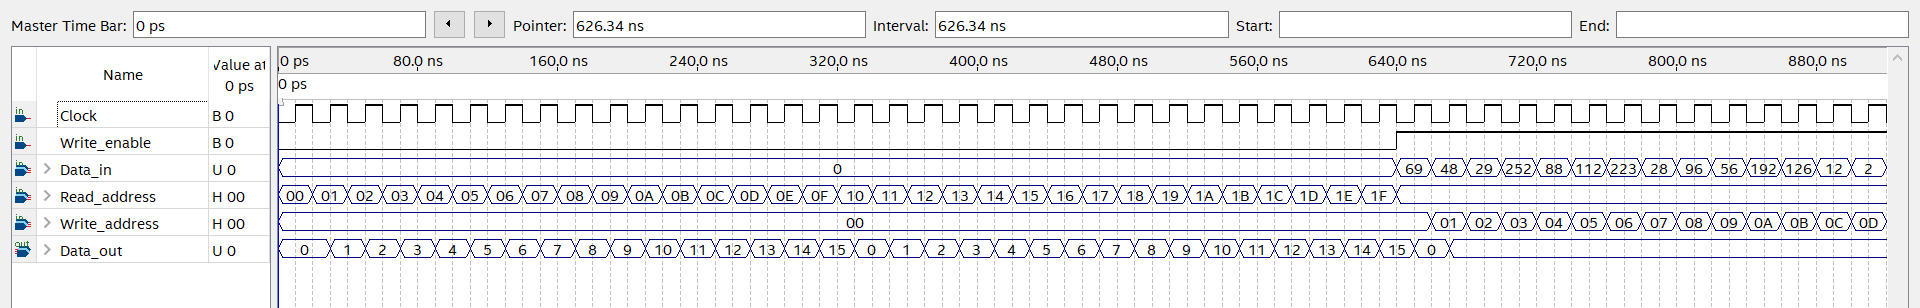
\includegraphics[scale = 0.4]{source/picture/Lab8/simulation_1.png}
    \caption{Simulation 1}
\end{figure}
\newpage
\begin{figure}[h]
    \centering
    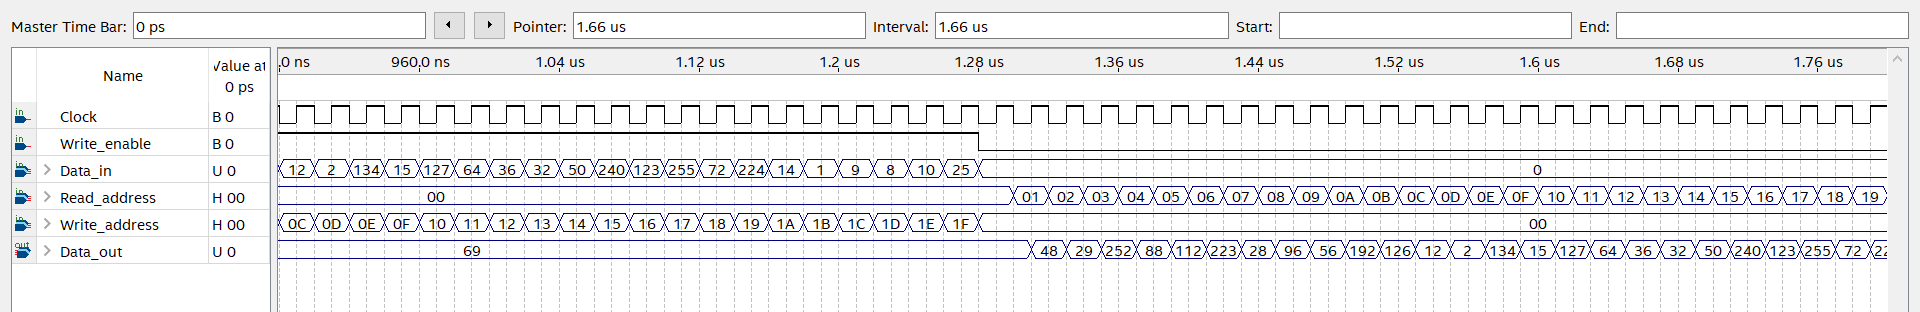
\includegraphics[scale = 0.4]{source/picture/Lab8/simulation_2.png}
    \caption{Simulation 2}
\end{figure}
\begin{figure}[h]
    \centering
    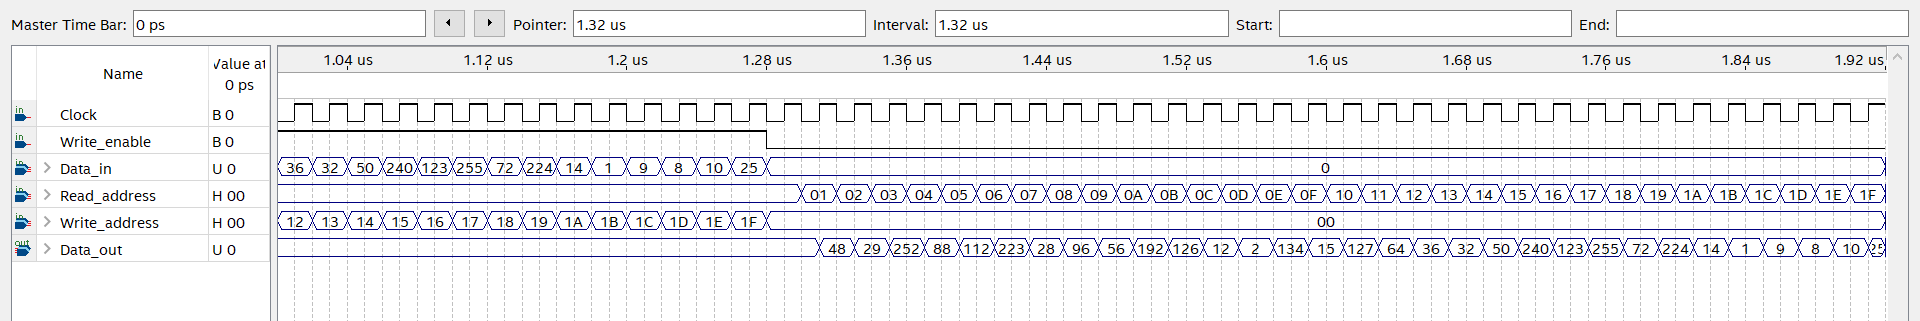
\includegraphics[scale = 0.4]{source/picture/Lab8/simulation_3.png}
    \caption{Simulation 3}
\end{figure}
The following is the code of ram 32x4.mif file which is initialized for the memory.
\begin{lstlisting}[language=Verilog]
DEPTH = 32;
WIDTH = 4;
ADDRESS_RADIX = HEX;
DATA_RADIX = BIN;
CONTENT
BEGIN
0  : 0000;
1  : 0001;
2  : 0010;
3  : 0011;
4  : 0100;
5  : 0101;
6  : 0110;
7  : 0111;
8  : 1000;
9  : 1001;
A  : 1010;
B  : 1011;
C  : 1100;
D  : 1101;
E  : 1110;
F  : 1111;
10 : 0000;
11 : 0001;
12 : 0010;
13 : 0011;
14 : 0100;
15 : 0101;
16 : 0110;
17 : 0111;
18 : 1000;
19 : 1001;
1A : 1010;
1B : 1011;
1C : 1100;
1D : 1101;
1E : 1110;
1F : 1111;
END;

\end{lstlisting}

\chap{ A Simple Processor}

\section{Introduction}
A \textbf{central processing unit (CPU)}, also called a \textbf{central processor}, \textbf{main processor} or just \textbf{processor}, is the electronic circuitry that executes instructions comprising a computer program. The CPU performs basic arithmetic, logic, controlling, and input/output (I/O) operations specified by the instructions in the program. This contrasts with external components such as main memory and I/O circuitry, and specialized processors such as graphics processing units (GPUs).\bigskip\\
The form, design, and implementation of CPUs have changed over time, but their fundamental operation remains almost unchanged. Principal components of a CPU include the arithmetic logic unit (ALU) that performs arithmetic and logic operations, processor registers that supply operands to the ALU and store the results of ALU operations, and a control unit that orchestrates the fetching (from memory), decoding and execution of instructions by directing the coordinated operations of the ALU, registers and other components.\bigskip\\
The following figure depicts the internals of a CPU.\\

\begin{figure}[h]
    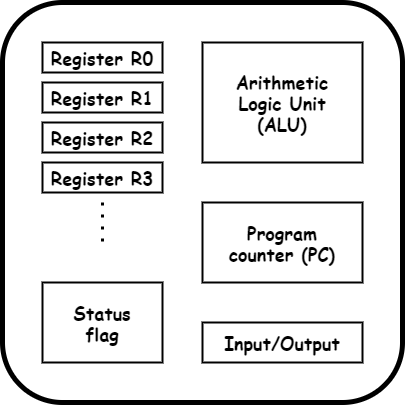
\includegraphics[scale = 0.5]{source/picture/Lab09/Processor_Image.png}
    \centering
\end{figure}

In which,
\begin{itemize}
	\item The \textbf{resistors} $R_0$, $R_1$, $R_2$, etc. are basically the CPU's internal RAM, and it will only have a small number of these. These resistors can either store numeric values or specific functions.
	\item The \textbf{arithmetic logic unit} is responsible for performing additions, subtractions, logic ands and ors, and other source of computation.
	\item The \textbf{status flags} registor is a collection of bits which will gives us information about the status of the CPU and the ALU.
	\item The \textbf{program counter} is used to store the address of where we are up to in our program. So, as the program is executed sequentially, the program counter increases. Furthermore, its value can be set depending on the result of something in the \textbf{status flags} register.
	\item \textbf{Input/Output} is how we are going to communicate, meaning getting the data in and out of the CPU.
\end{itemize}

\section{A Simple Processor}
The following figure shows a \textit{processor} that contains a number of nine-bit registers, a multiplexer, an adder/subtractor unit, and a control unit (finite state machine). Data is input to this system via the nine-bit DIN input. This data can be loaded through the nine-bit wide multiplexer into the various registers, such as $R_0$, . . . , $R_7$ and $A$. The multiplexer also allows data to be transferred from one register to another. The multiplexer’s output wires are called a bus in the figure because this term is often used for wiring that allows data to be transferred from one location in a system to another.\bigskip\\
Addition or subtraction of signed numbers is performed by using the multiplexer to first place one nine-bit number onto the bus wires and loading this number into register A. Once this is done, a second nine-bit number is placed onto the bus, the adder/subtractor unit performs the required operation, and the result is loaded into register G. The data in G can then be transferred to one of the other registers as required\\

\begin{figure}[h]
    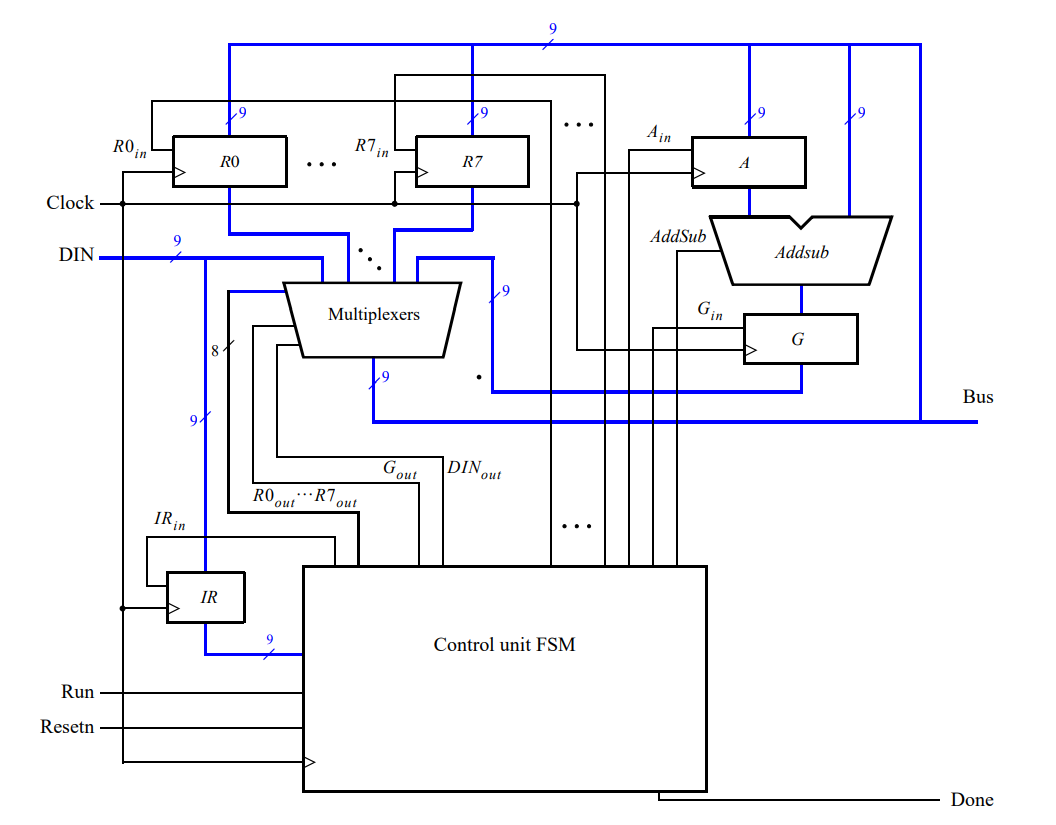
\includegraphics[scale = 0.75]{source/picture/Lab09/Simple_Processor_Figure.png}
    \centering
\end{figure}
\newpage

The system can perform different operations in each clock cycle, as governed by the control unit. This unit determines when particular data is placed onto the bus wires and it controls which of the registers is to be loaded with this data. For example, if the control unit asserts the signals $R0_{out}$ and $A_{in}$, then the multiplexer will place the contents of register $R_0$ onto the bus and this data will be loaded on the next active clock edge into $A$.\bigskip\\
The \textit{processor} executes operations specified in the form of \textit{instructions}. The following table lists the instructions the processor has to support. The left column shows the name of an instruction and its operands. The meaning of the syntax $Rx \xleftarrow{} [Ry]$ is that the contents of resister $Ry$ are loaded into register $Rx$. The \textbf{mv} (move) instruction allows data to be copied from one register to another. For the \textbf{mvi} (move immediate) instruction, the expression $Rx \xleftarrow{} D$ indicates that the nine-bit constant $D$ is loaded into register $Rx$.\\
\begin{table}[h]
    \begin{tabular}{l|l}
        Operation    & Function performed \\ \hline
        \textbf{mv} $Rx$,$Ry$   & $Rx \xleftarrow{} [Ry]$ \\ \hline
        \textbf{mvi} $Rx$,\#$D$ & $Rx \xleftarrow{} D$ \\ \hline
        \textbf{add} $Rx$,$Ry$  & $Rx\xleftarrow{}[Rx]+[Ry]$ \\ \hline
        \textbf{sub} $Ry$,$Ry$  & $Rx\xleftarrow{}[Rx]-[Ry]$
    \end{tabular}
    \centering
\end{table}

Each instruction can be encoded using the nine-bit format \textit{IIIXXXYYY} where \textit{III} specifies the instruction, \textit{XXX} gives the $Rx$ register, and \textit{YYY} gives the $Ry$ register. Although only two bits are needed to encode our four instructions, we are using three bits because other instructions will be added to the processor later. Assume that \textit{III} $=000$ for the \textbf{mv} instruction, 001 for \textbf{mvi}, 010 for \textbf{add}, and 011 for \textbf{sub}. Instructions are loaded from the the external input \textit{DIN}, and stored into the \textit{IR} register, using the connection indicated above. For the \textit{mvi} instruction, the \textit{YYY} field has no meaning, and the immediate data \#$D$ has to be supplied on the \textit{DIN} input in the clock cycle after the \textit{mvi} instruction word is stored into \textit{IR}.\bigskip\\
Some instructions, such as an addition or subtraction, take more than one clock cycle to complete, because multiple transfers have to be performed across the bus. The finite state machine in the control unit “steps through” such instructions, asserting the control signals needed in successive clock cycles until the instruction has completed. The processor starts executing the instruction on the \textit{DIN} input when the \textit{Run} signal is asserted and the processor asserts the \textit{Done} output when the instruction is finished. The following table indicates the control signals that can be asserted in each time step to implement the instructions in the previous table. Note that the only control signal asserted in time step 0 is \textit{IR}$_{in}$, so this time step is not shown in the table.\\
\begin{table}[h]
    \begin{tabular}{l|l|l|l}
     &\multicolumn{1}{c|}{T1}&\multicolumn{1}{c|}{T2}&\multicolumn{1}{c}{T3} \\ \hline
     (\textbf{mv}): $I_0$&$Ry_{out}$, $Rx_{in}$, \textit{done}&  &  \\ \hline
     (\textbf{mvi}): $I_1$&\textit{DIN}$_{out}$, $Rx_{in}$, \textit{done}&  &  \\ \hline
     (\textbf{add}): $I_2$&\textit{Rx}$_{out}$, $A_{in}$&\textit{Ry}$_{out}$, $G_{in}$&$G_{out}$, \textit{Rx}$_{in}$, \textit{done}\\ \hline
     (\textbf{sub}): $I_3$&\textit{Rx}$_{out}$, $A_{in}$&\textit{Ry}$_{out}$, $G_{in}$&$G_{out}$, \textit{Rx}$_{in}$, \textit{done} 
    \end{tabular}
    \centering
\end{table}
\newpage

The following block of \textbf{Verilog} code can be used to model the described processor.

\begin{lstlisting}[language=Verilog]
module pro(CLK,D_IN, RUN, RESET, DONE, BUS);
	input		[8:0]		D_IN;
	input					CLK, RESET, RUN;
	output	[8:0] 	BUS /*synthesis keep*/;
	output				DONE;
	
	wire		[8:0] 	reg0_out, reg1_out, reg2_out, reg3_out, reg4_out, reg5_out, reg6_out, reg7_out, regA_out, regG_out /*synthesis keep*/;
	wire		[8:0]		addsub_out /*synthesis keep*/;
	wire		[9:0]		reg_en /*synthesis keep*/;
	wire		[9:0]		multi_select /*synthesis keep*/;
	wire		[8:0] 	CODE /*synthesis keep*/;
	wire					MODE /*synthesis keep*/;
	
	regn	reg0 (.CLK(CLK), .EN(reg_en[0]), .IN(BUS), .OUT(reg0_out));
	regn	reg1 (.CLK(CLK), .EN(reg_en[1]), .IN(BUS), .OUT(reg1_out));
	regn	reg2 (.CLK(CLK), .EN(reg_en[2]), .IN(BUS), .OUT(reg2_out));
	regn	reg3 (.CLK(CLK), .EN(reg_en[3]), .IN(BUS), .OUT(reg3_out));
	regn	reg4 (.CLK(CLK), .EN(reg_en[4]), .IN(BUS), .OUT(reg4_out));
	regn	reg5 (.CLK(CLK), .EN(reg_en[5]), .IN(BUS), .OUT(reg5_out));
	regn	reg6 (.CLK(CLK), .EN(reg_en[6]), .IN(BUS), .OUT(reg6_out));
	regn	reg7 (.CLK(CLK), .EN(reg_en[7]), .IN(BUS), .OUT(reg7_out));
	regn	regA (.CLK(CLK), .EN(reg_en[8]), .IN(BUS), .OUT(regA_out));
	regn	regG (.CLK(CLK), .EN(reg_en[9]), .IN(addsub_out), .OUT(regG_out));
	regn	regI (.CLK(CLK), .EN(RUN), .IN(D_IN), .OUT(CODE));
	
	multiplexer inst0 (.IN0(reg0_out), .IN1(reg1_out), .IN2(reg2_out), .IN3(reg3_out), .IN4(reg4_out), 
							 .IN5(reg5_out), .IN6(reg6_out), .IN7(reg7_out), .IN8(regG_out), .IN9(D_IN), 
							 .SELECT(multi_select), .OUT(BUS));
							 
	addsub		inst1 (.MODE(MODE), .IN0(regA_out), .IN1(BUS), .OUT(addsub_out));
	
	control		inst2	(.CLK(CLK), .RUN(RUN), .RESET(RESET), .DONE(DONE), .CODE(CODE),
							 .REG_EN(reg_en), .MULTI_SELECT(multi_select), .MODE(MODE));
endmodule

module control(CLK, CODE, RUN, RESET, DONE, MODE, REG_EN, MULTI_SELECT);
	parameter MV=3'b000, MVI=3'b001, ADD=3'b010, SUB=3'b011, LDY=3'b100, UDX=3'b101, LDI=3'b110;  
	input		[8:0]		CODE;
	input					RUN, RESET, CLK;
	
	output	reg [9:0]	REG_EN;
	output	reg [9:0]	MULTI_SELECT;
	output	reg			DONE, MODE;
	
	reg		[2:0]		fsm_in, fsm_out /*synthesis keep */;

	
	//FSM
	always @(posedge CLK) begin
		fsm_out <= fsm_in;
	end
	
	always @(CODE) begin
		case (fsm_out)
			MV: fsm_in = CODE [8:6];
			MVI:fsm_in = LDI;
			ADD:fsm_in = LDY;
			SUB:fsm_in = LDY;
			LDY:fsm_in = UDX;
			UDX:fsm_in = CODE [8:6];
			default: fsm_in = CODE [8:6];
		endcase
	end
	
	//Control
	always @(fsm_in) begin
			if (fsm_in==MV) begin 
				MULTI_SELECT = {10{1'b0}} | (1<<CODE[2:0]);
				REG_EN 		 = {10{1'b0}} | (1<<CODE[5:3]);
				DONE			 = 1 ;
			end else 
			if (fsm_in==MVI) begin
				MULTI_SELECT = {10{1'b0}} | (1<<9);
				REG_EN 		 = {10{1'b0}} | (1<<CODE[5:3]);
				DONE			 = 0 ;
			end else
			if (fsm_in==LDI) begin
				REG_EN 		 = {10{1'b0}} | (0<<CODE[5:3]);
				DONE			 = 1 ;
			end else 
			if (fsm_in==ADD | fsm_in==SUB) begin
				MULTI_SELECT = {10{1'b0}} | (1<<CODE[5:3]);
				REG_EN 		 = {10{1'b0}} | (1<<8);
				DONE			 = 0 ;
			end else 
			if (fsm_in==LDY) begin
				MULTI_SELECT = {10{1'b0}} | (1<<CODE[2:0]);
				REG_EN 		 = {10{1'b0}} | (1<<9);
				DONE			 = 0 ;
			end else
			if (fsm_in==UDX) begin
				MULTI_SELECT = {10{1'b0}} | (1<<8);
				REG_EN 		 = {10{1'b0}} | (1<<CODE[5:3]);
				DONE			 = 1 ; 
			end
			
			if (fsm_in==ADD) MODE = 1'b0 ;
			if (fsm_out==SUB)MODE = 1'b1 ;
			
		end

endmodule

module multiplexer(IN0, IN1, IN2, IN3, IN4, IN5, IN6, IN7, IN8, IN9, SELECT, OUT);
	input		[8:0] 	IN0, IN1, IN2, IN3, IN4, IN5, IN6, IN7, IN8, IN9;
	input		[9:0]		SELECT;
	output	[8:0]		OUT /*synthesis keep*/;
	
	assign	OUT = IN0 & {9{SELECT[0]}} |
						IN1 & {9{SELECT[1]}} |
						IN2 & {9{SELECT[2]}} |
						IN3 & {9{SELECT[3]}} |
						IN4 & {9{SELECT[4]}} |
						IN5 & {9{SELECT[5]}} |
						IN6 & {9{SELECT[6]}} |
						IN7 & {9{SELECT[7]}} |
						IN8 & {9{SELECT[8]}} |
						IN9 & {9{SELECT[9]}} ;
endmodule

module addsub(MODE, IN0, IN1, OUT);
	parameter ADD=1'b0, SUB=1'b1;
	
	input		[8:0]	IN0, IN1 /*synthesis keep*/;
	input				MODE;
	output 	reg[8:0]	OUT;
	
	
	always @(IN0, IN1) begin
		if (MODE==ADD) OUT = IN1 + IN0;
		else OUT = IN1 - IN0;
	end
	
	
endmodule

module regn(IN, EN, CLK, OUT);
parameter n = 9;
	input 	[n-1:0] IN;
	input 	EN, CLK;
	output 	reg [n-1:0] OUT;
		
	always @(posedge CLK)
		if (EN)
			OUT <= IN;
endmodule
\end{lstlisting}

Using \textbf{Quartus}, we can generate a schematic block diagram and a waveform simulation, and the results are as followed.

\begin{figure}[h]
    \centering
    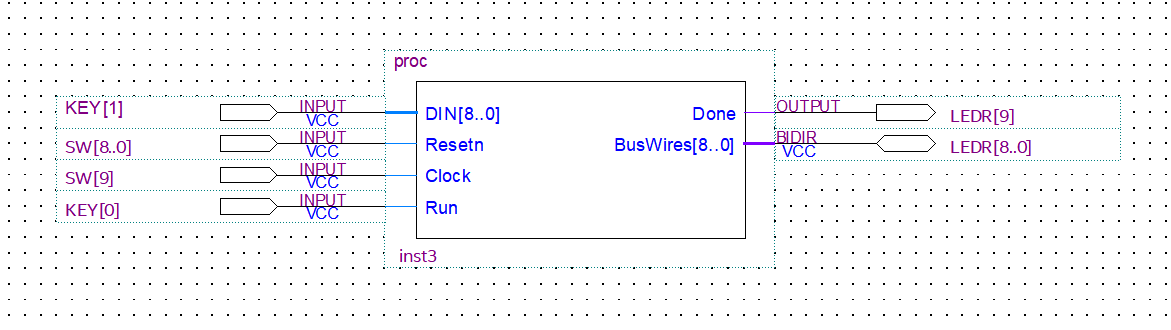
\includegraphics[scale = 0.5]{source/picture/Lab09/Lab9_1.png}
\end{figure}
\clearpage
\begin{figure}[h]
    \centering
    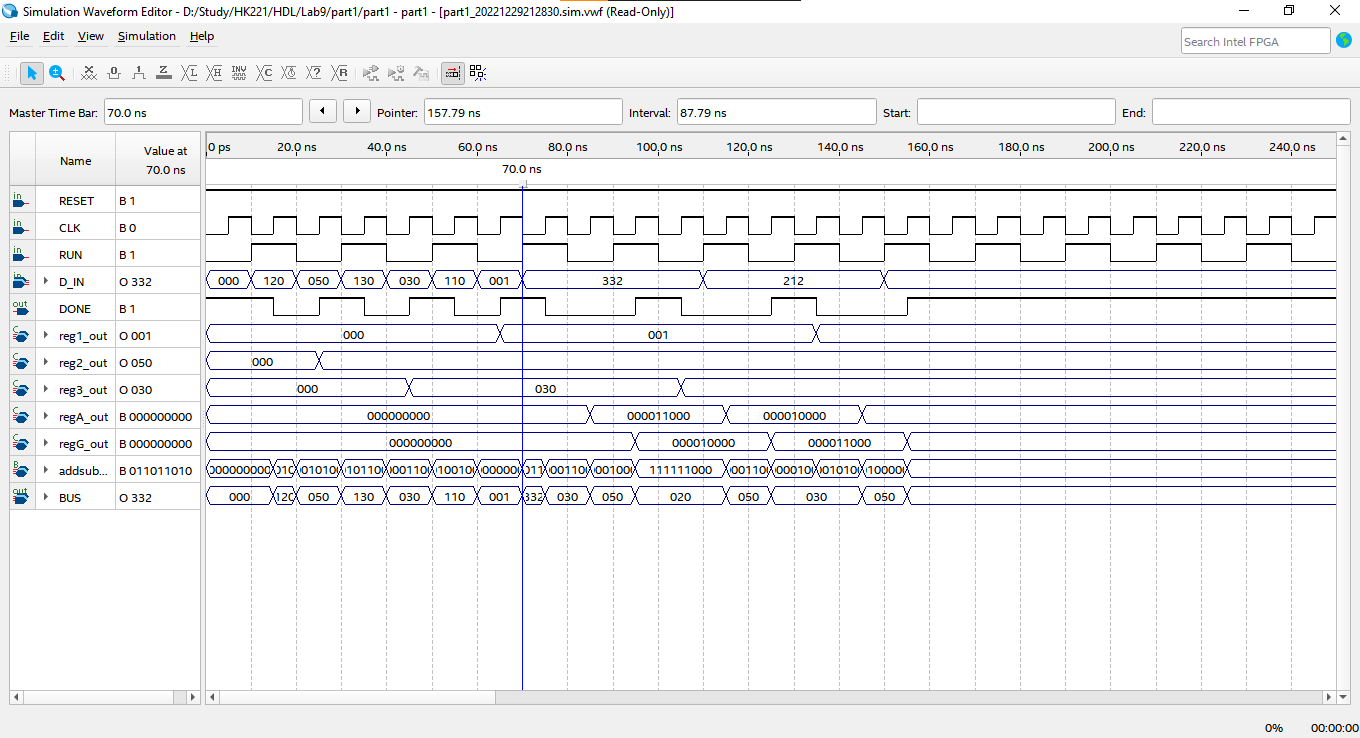
\includegraphics[width = \textwidth]{source/picture/Lab09/Lab9_1_stimulation.png}
\end{figure}

Here are some explanations for the simulation result above:
\begin{itemize}
    \item At $t=10ns$, the instruction 120 (9'b001010000) $\iff$ "\textbf{mvi} R2" is loaded into processor via \textbf{Run} signal, then at $t=15ns$ it is executed \textbf{Run} signal. In the next clock pulse (at $t=25ns$), the \textbf{value 050 is loaded into R2} and the signal \textbf{Done} is immediately returned. \textbf{This operation takes 2 clock pulses to complete.}
    \item At $t=20ns$, the instruction 120 (9'b001011000) $\iff$ "\textbf{mvi} R3" is loaded into processor via \textbf{Run} signal, then at $t=25ns$ it is executed. In the next clock pulse (at $t=35ns$), the \textbf{value 050 is loaded into R2} and the signal \textbf{Done} is immediately returned. \textbf{This operation takes 2 clock pulses to complete.}
    \item At $t=50ns$, the instruction 110 (9'b001001000) $\iff$ "\textbf{mvi} R1" is loaded into BUS\_WIRE, then at $t=55ns$ flows to the processor via the \textbf{Run} signal. In the next clock pulse (at $t=65ns$), the \textbf{value 001 is loaded into R1} and the signal \textbf{Done} is immediately returned. \textbf{This operation takes 2 clock pulses to complete.}
    \item At $t=70ns$, the instruction 332 (9'b011011010) $\iff$ "\textbf{sub} R3,R2" is loaded into processor via \textbf{Run} signal, then it is executed at $t=75ns$ - this is the reason why at this time, the BUS\_WIRE hold the value of R3 (020), immediately, this value flows to the \textbf{Addsub} module. At the next clock pulse, the value of the $R_2$ (050) is loaded into the BUS\_WIRE, then flow to {Addsub} to compute the value, in this case, this module minus 020 from 050 and save into $R_3$. This operation takes 3 clock pulses to complete.
\end{itemize}
\clearpage
Let's take this one step further by adding a memory module and a counter to our processor. The counter is used to read the contents of successive addresses in the memory, and this data is provided to the processor as a stream of instructions. To simplify the design and testing of this circuit we will use separate clock signals, PClock and MClock, for the processor and the memory.

\begin{figure}[h]
    \centering
    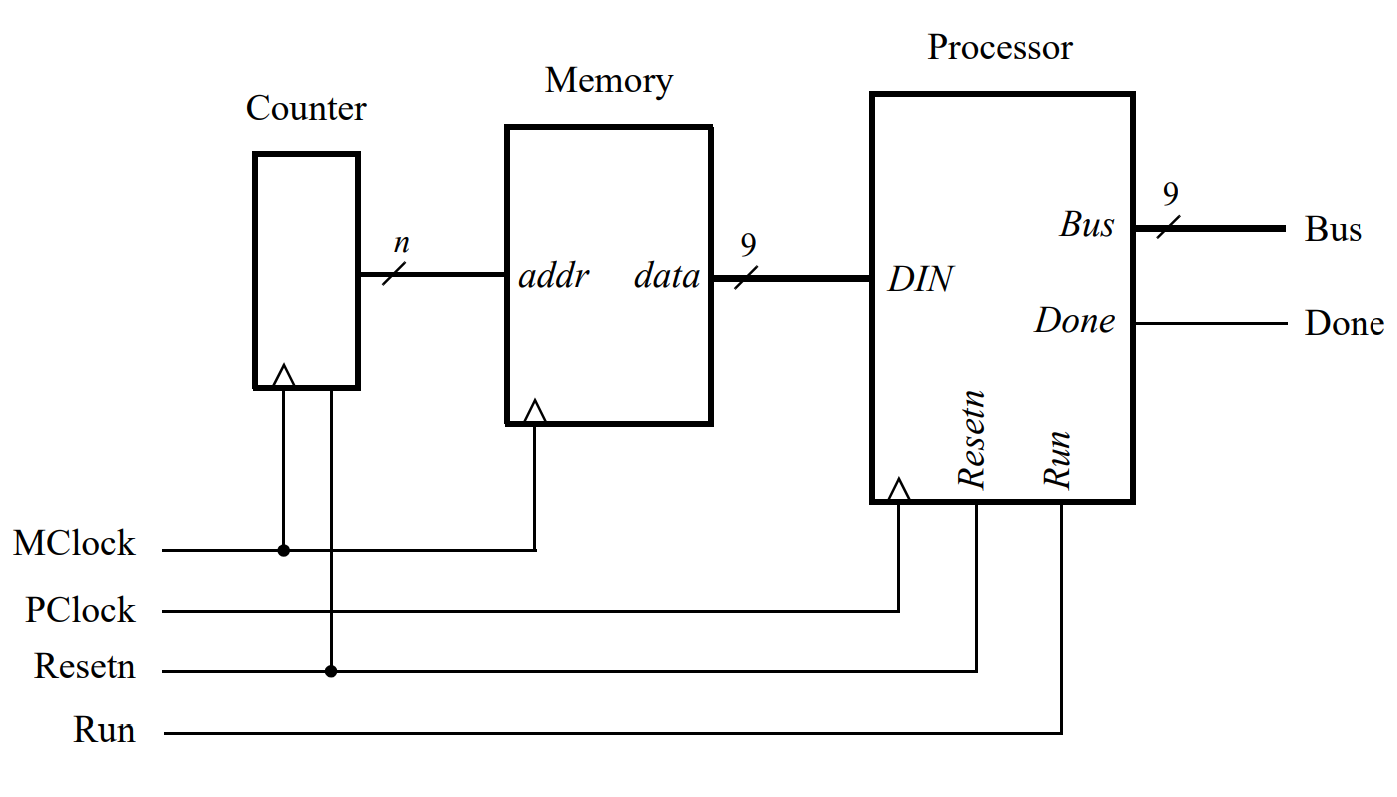
\includegraphics[width=5.5in]{source/picture/Lab09/Simple_Processor_W_Counter.png}
\end{figure}

The counter we will be using is just a simple mod-32 counter. The \textbf{verilog} code for the counter is as followed.

\begin{lstlisting}[language=Verilog]
module counterv(CLK,RESET,Q);
	input CLK,RESET;
	output reg [4:0] Q;
	
	
	always@(posedge CLK) begin
		if(!RESET) Q<=0;
		else Q<=Q+1;
	end
	
endmodule
\end{lstlisting}

Next, the memory we will be using will be called a \textit{synchronous read-only memory (synchronous ROM)} since it has only a read port and no write port. Using the Quartus IP Catalog tool, we can create this memory module as follow.

\begin{figure}[h]
    \centering
    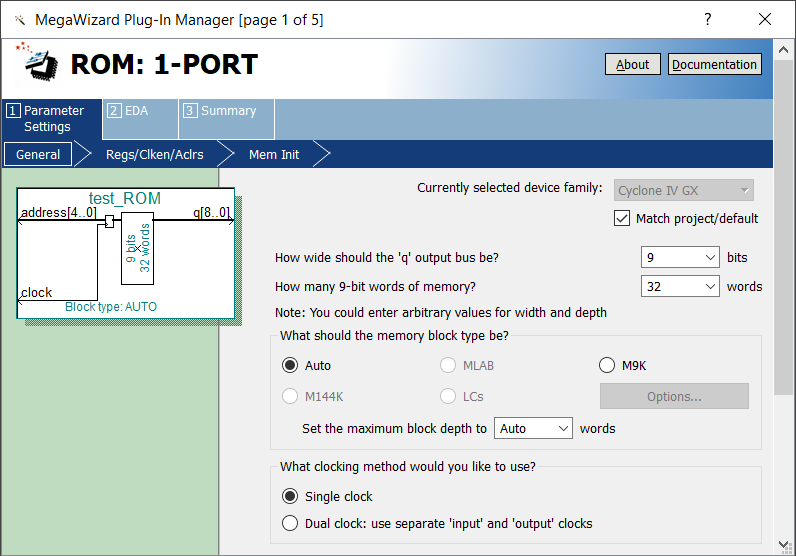
\includegraphics[width = 5.5in]{source/picture/Lab09/Create_ROM_1.png}
\end{figure}

\begin{figure}[h]
    \centering
    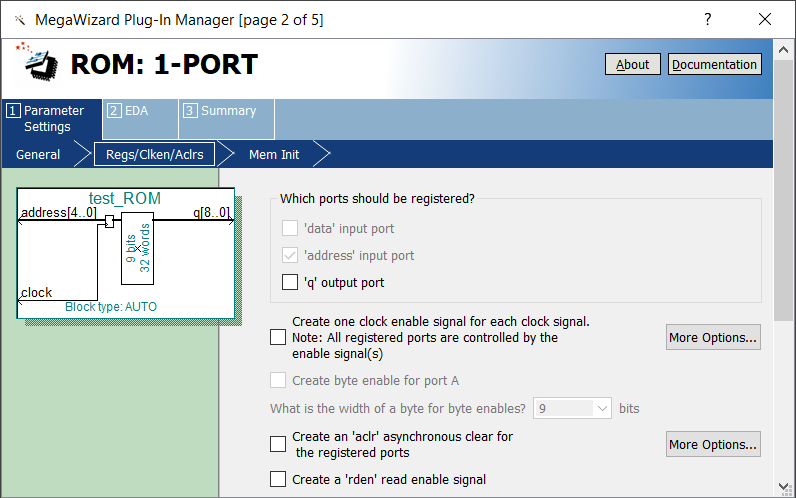
\includegraphics[width = 5.5in]{source/picture/Lab09/Create_ROM_2.png}
\end{figure}

We can initialize the initial content of the memory by using a \textit{Memory Initialization File} [.mif]. So we created such file, named \textit{inst\_mem.mif} and its content is as followed.
\newpage

\begin{lstlisting}[language=verilog]

WIDTH=9;
DEPTH=32;

ADDRESS_RADIX=UNS;
DATA_RADIX=OCT;

CONTENT BEGIN
    0   :   100;
    1   :   005;
    2   :   010;
    3   :   201;
    4   :   300;
    [5..31]  :   000;
END;
\end{lstlisting}

\newpage

Using \textbf{Quartus}, we can generate a schematic block diagram and a waveform simulation. The results are as followed. (Click \href{https://drive.google.com/file/d/1bG-vFAlYrJjy5utJ4DoETYb3e9kJMEU5/view?usp=sharing}{here} for a more detailed schematic and \href{https://drive.google.com/file/d/1yXu4M1fxIND9-f9YMr3JbLg8KXuOInd-/view?usp=sharing}{here} for a more detailed simulation result)

\begin{figure}[h]
    \centering
    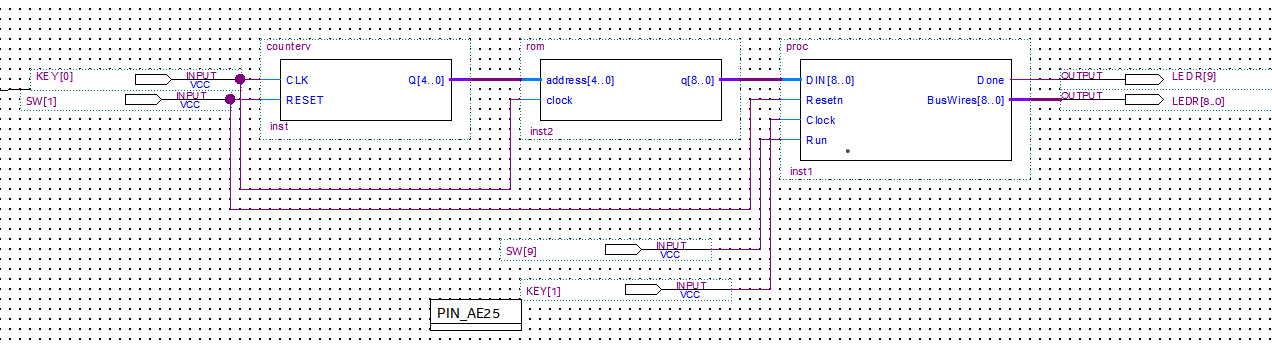
\includegraphics[width=6.1in]{source/picture/Lab09/Lab9_2.png}
\end{figure}

\begin{figure}[h]
    \centering
    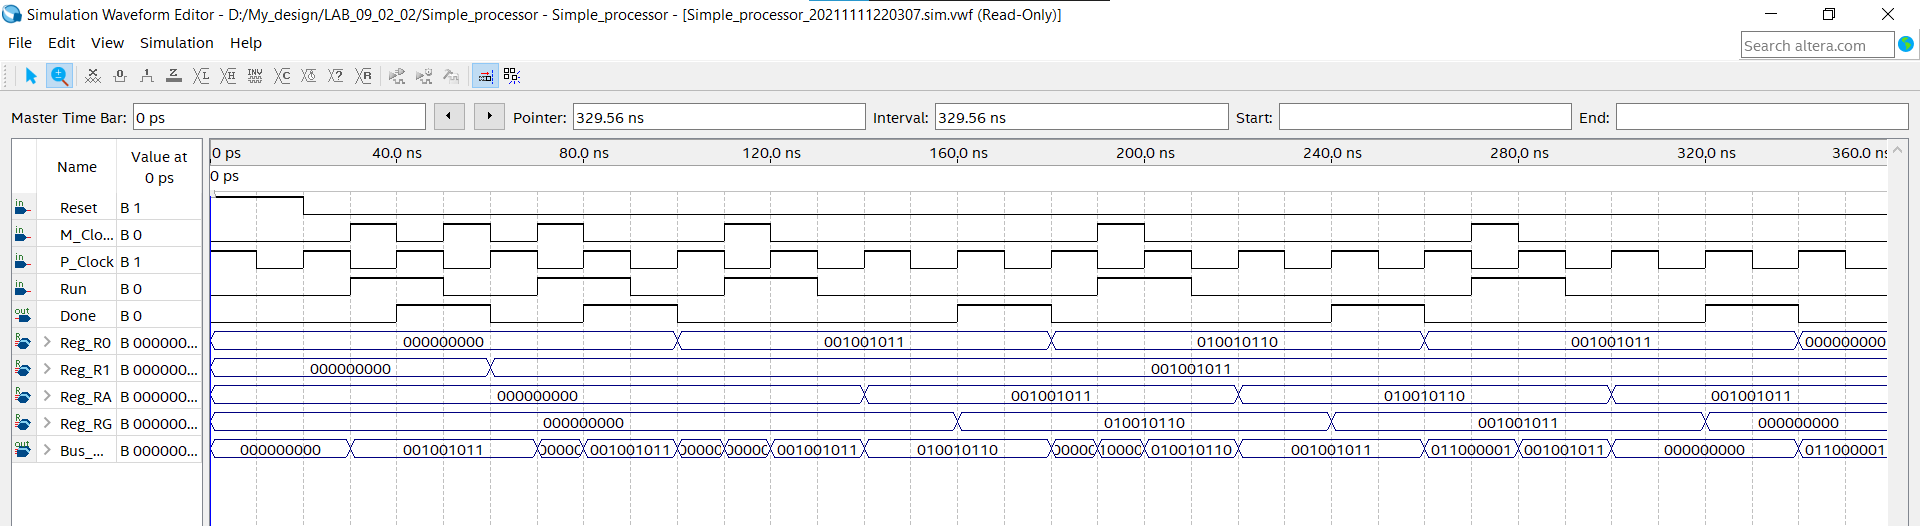
\includegraphics[width=6.1in]{source/picture/Lab09/Simple_Processor_W_Counter_Simulation.png}
\end{figure}

Here are some explanations for the simulation result above:
\begin{itemize}
    \item The instructions and instruction order are exactly the same as with the previous simulation result. The interesting thing here is the way that we load the instruction to our processor. Therefore, we will focus more on that aspect.
    \item At $t=30ns$, there is an \textbf{M\_Clock} signal to start both the counter and the ROM. After this, we are at the address 00 : 001001011. Then there's a \textbf{Run} signal and the processor loads the instruction 001001011 in.
    \item At $t=50ns$, another \textbf{M\_Clock} signal moves us to the next address 01 : 001001011. The processor then proceeds to load the value 001001011 into the $R_1$ register.
    \item At $t=70ns$, another \textbf{M\_Clock} signal moves us to the next address 02 : 000000001. The processor then proceeds to load the value of register $R_1$ into register $R_0$.
    \item At $t=110ns$, another \textbf{M\_Clock} signal moves us to the next address 03 : 010000001. The processor then proceeds to add the value of registers $R_1$ and $R_0$ together, then registers that value into $R_0$.
    \item At $t=190ns$, another \textbf{M\_Clock} signal moves us to the next address 04 : 011000001. The processor then proceeds to subtracts the value of registers $R_1$ from $R_0$, then registers that value into $R_0$.
    \item At $t=270ns$, another \textbf{M\_Clock} signal moves us to the next address 05 : 011000001. The processor then proceeds to subtracts the value of registers $R_1$ from $R_0$, then registers that value into $R_0$.
\end{itemize}
%\chap{ An Enhanced Processor}

\section{Part 3}
In this part you will extend the capability of the processor so that the external counter is no longer needed, and so
that the processor has the ability to perform read and write operations using memory or other devices. You will
add three new types of instructions to the processor, as displayed in Table 3. The ld (load) instruction loads data
into register RX from the external memory address specified in register RY. The st (store) instruction stores the
data contained in register RX into the memory address found in RY. Finally, the instruction mvnz (move if not
zero) allows a mv operation to be executed only under the condition that the current contents of register G are not
equal to 0.\\
\begin{figure}[h]
    \centering
    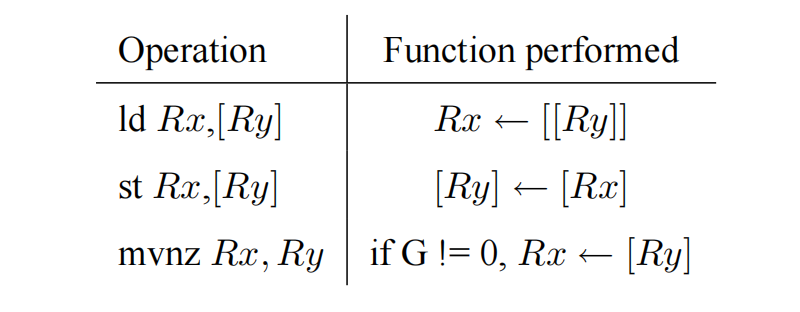
\includegraphics[scale = 0.6]{source/picture/Lab10/pic1.png}
\end{figure}

A schematic of the enhanced processor is given in Figure 11. In this figure, registers R0 to R6 are the same
as in Figure 1 of Laboratory Exercise 9, but register R7 has been changed to a counter. This counter is used
to provide the addresses in the memory from which the processor’s instructions are read; in the preceding lab
exercise, a counter external to the processor was used for this purpose. We will refer to R7 as the processor’s
program counter (PC), because this terminology is common for real processors available in the industry. When
the processor is reset, PC is set to address 0. At the start of each instruction (in time step 0) the contents of PC
are used as an address to read an instruction from the memory. The instruction is stored in IR and the PC is
automatically incremented to point to the next instruction (in the case of mvi the PC provides the address of the
immediate data and is then incremented again).\\
The processor’s control unit increments PC by using the $incr_PC$ signal, which is just an enable on this counter. It
is also possible to directly load an address into PC (R7) by having the processor execute a mv or mvi instruction
in which the destination register is specified as R7. In this case the control unit uses the signal R7in to perform
a parallel load of the counter. In this way, the processor can execute instructions at any address in memory, as
opposed to only being able to execute instructions that are stored in successive addresses. Similarly, the current
contents of PC can be copied into another register by using a mv instruction. An example of code that uses the
PC register to implement a loop is shown below, where the text after the \% on each line is just a comment. The
instruction mv R5,R7 places into R5 the address in memory of the instruction sub R4,R2. Then, the instruction
mvnz R7,R5 causes the sub instruction to be executed repeatedly until R4 becomes 0. This type of loop could be
used in a larger program as a way of creating a delay\\
\begin{figure}[h]
    \centering
    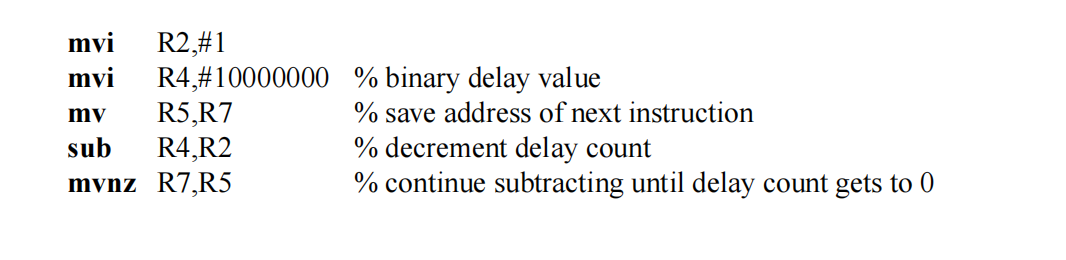
\includegraphics[scale = 0.6]{source/picture/Lab10/pic2.png}
\end{figure}
\newpage
Figure 11 shows two registers in the processor that are used for data transfers. The ADDR register is used to send
addresses to an external device, such as a memory module, and the DOUT register is used by the processor to
provide data that can be stored outside the processor. One use of the ADDR register is for reading, or fetching, instructions from memory; when the processor wants to fetch an instruction, the contents of PC (R7) are transferred
across the bus and loaded into ADDR. This address is provided to memory. In addition to fetching instructions,
the processor can read data at any address by using the ADDR register. Both data and instructions are read into the
processor on the DIN input port. The processor can write data for storage at an external address by placing this
address into the ADDR register, placing the data to be stored into its DOUT register, and asserting the output of
the W (write) flip-flop to 1.\\
Figure 12 illustrates how the enhanced processor is connected to memory and other devices. The memory unit
in the figure supports both read and write operations and therefore has both address and data inputs, as well as a
write enable input. The memory also has a clock input, because the address, data, and write enable inputs must be
loaded into the memory on an active clock edge. This type of memory unit is usually called a synchronous static
random access memory (synchronous SRAM). Figure 12 also includes a 9-bit register that can be used to store data
2
ADDR DOUT
from the processor; this register might be connected to a set of LEDs to allow display of data on your DE-series
board. To allow the processor to select either the memory unit or register when performing a write operation, the
circuit includes some logic gates that perform address decoding: if the upper address lines are A8A7 = 00, then
the memory module will be written at the address given on the lower address lines. Figure 12 shows n lower
address lines connected to the memory; for this exercise a memory with 128 words is probably sufficient, which
implies that n = 7 and the memory address port is driven by A6 . . . A0. For addresses in which A8A7 = 01, the
data written by the processor is loaded into the register whose outputs are called LEDs in Figure 12.\\
\begin{figure}[h]
    \centering
    \includegraphics[scale = 0.5]{source/picture/Lab10/pic3.png}
\end{figure}

1. Create a new Quartus project for the enhanced version of the processor.\\
2. Write Verilog code for the processor and test your circuit by using functional simulation: apply instructions
to the DIN port and observe the internal processor signals as the instructions are executed. Pay careful
attention to the timing of signals between your processor and external memory; account for the fact that the
memory has registered input ports, as we discussed for Figure 12.\\
3. Create another Quartus project that instantiates the processor, memory module, and register shown in Figure 12. Use the Quartus IP Catalog to create the RAM: 1-PORT memory module. Follow the instructions
provided by the wizard to create a memory that has one 9-bit wide read/write data port and is 128 words
deep. Ensure that the output is not registered. Use a MIF file to store instructions in the memory that are to
be executed by your processor. An example program in the form of a MIF file is shown in Figure 13. This
program display an 8-bit counter value on the LEDs output port. Loops are used in the program to create
delays so that the counter values are not changed too quickly to be observed. Comments are included in the
MIF file in Figure 13 to describe the program’s code.\\
4. Use functional simulation to test the circuit. Ensure that data is read properly from the memory and executed
by the processor.\\
5. Include in your project the necessary pin assignments to implement your circuit on your DE-series board.
Use switch SW9 to drive the processor’s Run input, use KEY0 for Resetn, and use the board’s 50 MHz
clock signal as the Clock input. Since the circuit needs to run properly at 50 MHz, make sure that a timing
constraint is set in Quartus to constrain the circuit’s clock to this frequency. Read the Report produced
by the Quartus Timing Analyzer to ensure that your circuit operates at this speed; if not, use the Quartus
tools to analyze your circuit and modify your Verilog code to make a more efficient design that meets the
3
Resetn
Run
50-MHz speed requirement. Also note that the Run input is asynchronous to the clock signal, so make sure
to synchronize this input using flip-flops.\\
Connect the LEDs register in Figure 12 to $LEDR_{8-0}$ so that you can observe the output produced by the
processor\\
\newpage
\lstdefinestyle{verilog-style}
{
    language=Verilog,
    basicstyle=\small\ttfamily,
    keywordstyle=\color{vblue},
    identifierstyle=\color{black},
    commentstyle=\color{vgreen},
    numbers=left,
    numberstyle=\tiny\color{black},
    numbersep=10pt,
    tabsize=8,
    moredelim=*[s][\colorIndex]{[}{]},
    literate=*{:}{:}1
}
\definecolor{vgreen}{RGB}{104,180,104}
\definecolor{vblue}{RGB}{49,49,255}
\definecolor{vorange}{RGB}{255,143,102}

\makeatletter
\newcommand*\@lbracket{[}
\newcommand*\@rbracket{]}
\newcommand*\@colon{:}
\newcommand*\colorIndex{%
    \edef\@temp{\the\lst@token}%
    \ifx\@temp\@lbracket \color{black}%
    \else\ifx\@temp\@rbracket \color{black}%
    \else\ifx\@temp\@colon \color{black}%
    \else \color{vorange}%
    \fi\fi\fi
}
\makeatother


\subsection{Code, memory and Simulation}
\begin{lstlisting}[style={verilog-style}]
module part3 ( W,BusWires,ADDR,SW, KEY, LEDR,Tstep ,EN,Done);  //Main part Run
  # Initial Variable
  input EN;
  input [8:0] SW;
  input [2:0] KEY;
  output reg [8:0] LEDR;
  output [2:0] Tstep;
  output Done;
  wire [8:0] DIN, DOUT, LEDsOUT;
  wire Resetn, Clock, Run;
  output W;
  output [8:0]BusWires,ADDR;
  reg LEDen, MEMen;

  assign MClock = KEY[1];
  assign PClock = KEY[2];

  assign Resetn = KEY[0];
  
  wire [8:0] R0;
  always
    if (EN)
      LEDR[8:0] = DIN;
    else
      LEDR[8:0] = R0;
  
  always
  begin
    LEDen = W & ~( ADDR[8] | ~ADDR[7]);
    MEMen = W & ~( ADDR[8] | ADDR[7]);
  end
  
  proc P0 (DIN, Resetn, PClock, Run, Done, BusWires, ADDR, DOUT, W, Tstep[2:0], R0);
  regn LEDs (DOUT, LEDen, MClock, LEDsOUT);
  Me Memory (ADDR, MClock, DOUT, MEMen, DIN);

endmodule

//The main processor
module processor (DIN, Resetn, Clock, Run, Done, BusWires, ADDR,
DOUT, W, Tstep_Q, R0);
  input [8:0] DIN;
  input Resetn, Clock, Run;
  output reg Done;
  output reg [8:0] BusWires;
  output [8:0] ADDR, DOUT;
  output W;
  output [2:0] Tstep_Q;
  output [8:0] R0;
 // output [8:0] A, G;
  //declare variables
  reg IRin, DINout, Ain, Gout, Gin, AddSub, incr_pc, ADDRin, DOUTin, W_D;
  reg [7:0] Rout, Rin;
  wire [7:0] Xreg, Yreg;
  wire [1:9] IR;
  wire [1:3] I;
  reg [9:0] MUXsel;
  wire [8:0] R0, R1, R2, R3, R4, R5, R6, R7, result;
  wire [8:0] A, G;
  wire [2:0] Tstep_Q;

  wire Clear = Done | ~Resetn;
  upcount Tstep (Clear, Clock, Tstep_Q);
  assign I = IR[1:3];
  dec3to8 decX (IR[4:6], 1'b1, Xreg);
  dec3to8 decY (IR[7:9], 1'b1, Yreg);
  always @(Tstep_Q or I or Xreg or Yreg)
  begin
    //specify initial values
    IRin = 1'b0;
    Rout[7:0] = 8'b00000000;
    Rin[7:0] = 8'b00000000;
    DINout = 1'b0;
    Ain = 1'b0;
    Gout = 1'b0;
    Gin = 1'b0;
    AddSub = 1'b0;
    DOUTin = 1'b0;
    ADDRin = 1'b0;
    W_D = 1'b0;
    incr_pc = 1'b0;

    Done = 1'b0;

    case (Tstep_Q)
      3'b000: // load next instruction in time step 0
      begin
        Rout = 8'b00000001;
        ADDRin = 1'b1;
        incr_pc = 1'b1;
		  IRin = 1'b1;
      end
      3'b001: //define signals in time step 1
        case (I)
          3'b000: // mv
          begin
            Rout = Yreg;
            Rin = Xreg;
            Done = 1'b1;
          end
          3'b001: // mvi
          begin
            DINout = 1'b1;
            Rin = Xreg;
            Done = 1'b1;
            incr_pc = 1'b1;
          end
          3'b010: // add
          begin
            Rout = Xreg;
            Ain = 1'b1;
          end
          3'b011: // sub
          begin
            Rout = Xreg;
            Ain = 1'b1;
          end
          3'b100: // ld
          begin
            Rout = Yreg;
            ADDRin = 1'b1;
          end
          3'b101: // st
          begin
            Rout = Xreg;
            DOUTin = 1'b1;
          end
          3'b110: // mvnz
          begin
            if (G != 0) begin
              Rout = Yreg;
              Rin = Xreg;
            end
            Done = 1'b1;
          end
        endcase
      3'b010: //define signals in time step 2
        case (I)
          3'b010: // add
          begin
            Rout = Yreg;
            Gin = 1'b1;
				AddSub = 1'b1;
          end
          3'b011: // sub
          begin
            Rout = Yreg;
            Gin = 1'b1;
            AddSub = 1'b1;
          end
          3'b100: // ld
          begin
            DINout = 1'b1;
            Rin = Xreg;
            Done = 1'b1;
          end
          3'b101: // st
          begin
            Rout = Yreg;
            ADDRin = 1'b1;
            W_D = 1'b1;
				//Done = 1'b1;
          end
        endcase
      3'b011: //define signals in time step 3
        case (I)
          3'b010: // add
          begin
            Gout = 1'b1;
            Rin = Xreg;
            Done = 1'b1;
          end
          3'b011: // sub
          begin
            Gout = 1'b1;
            Rin = Xreg;
            Done = 1'b1;
          end
        endcase
    endcase
  end

  //instantiate registers and the adder/subtracter unit

  counter reg_0 (1'b1, Clock, incr_pc, BusWires, ~Resetn, Rin[0], R0);
  regn reg_1 (BusWires, Rin[1], Clock, R1);
  regn reg_2 (BusWires, Rin[2], Clock, R2);
  regn reg_3 (BusWires, Rin[3], Clock, R3);
  regn reg_4 (BusWires, Rin[4], Clock, R4);
  regn reg_5 (BusWires, Rin[5], Clock, R5);
  regn reg_6 (BusWires, Rin[6], Clock, R6);
  regn reg_7 (BusWires, Rin[7], Clock, R7);

  regn reg_IR (DIN, IRin, Clock, IR);
  defparam reg_IR.n = 9;
  regn reg_A (BusWires, Ain, Clock, A);
  regn reg_G (result, Gin, Clock, G);

  regn reg_ADDR (BusWires, ADDRin, Clock, ADDR);
  regn reg_DOUT (BusWires, DOUTin, Clock, DOUT);
  regn reg_W (W_D, 1'b1, Clock, W);
  defparam reg_W.n = 1; 

  add_sub AS (~AddSub, A, BusWires, result);

  //define the bus
  always @ (MUXsel or Rout or Gout or DINout)
  begin
    MUXsel[9:2] = Rout;
    MUXsel[1] = Gout;
    MUXsel[0] = DINout;
    
    case (MUXsel)
      10'b0000000001: BusWires = DIN;
      10'b0000000010: BusWires = G;
      10'b0000000100: BusWires = R0;
      10'b0000001000: BusWires = R1;
      10'b0000010000: BusWires = R2;
      10'b0000100000: BusWires = R3;
      10'b0001000000: BusWires = R4;
      10'b0010000000: BusWires = R5;
      10'b0100000000: BusWires = R6;
      10'b1000000000: BusWires = R7;
    endcase
  end

endmodule


module upcount(Clear, Clock, Q);
  input Clear, Clock;
  output [2:0] Q;
  reg [2:0] Q;

  always @(posedge Clock)
    if (Clear)
      Q <= 3'b0;
    else
      Q <= Q + 1'b1;
endmodule

module dec3to8(W, En, Y);
  input [2:0] W;
  input En;
  output [0:7] Y;
  reg [0:7] Y;

  always @(W or En)
  begin
    if (En == 1)
      case (W)
        3'b000: Y = 8'b10000000;
        3'b001: Y = 8'b01000000;
        3'b010: Y = 8'b00100000;
        3'b011: Y = 8'b00010000;
        3'b100: Y = 8'b00001000;
        3'b101: Y = 8'b00000100;
        3'b110: Y = 8'b00000010;
        3'b111: Y = 8'b00000001;
      endcase
    else
      Y = 8'b00000000;
  end
endmodule


module regn(R, Rin, Clock, Q);
  parameter n = 9;
  input [n-1:0] R;
  input Rin, Clock;
  output [n-1:0] Q;
  reg [n-1:0] Q;

  always @(posedge Clock)
    if (Rin)
      Q <= R;
endmodule

module counter_modk(clock, reset_n, Q);
  parameter n = 4;
  parameter k = 16;

  input clock, reset_n;
  output [n-1:0] Q;
  reg [n-1:0] Q;

  always @(posedge clock or negedge reset_n)
  begin
    if (~reset_n)
      Q <= 'd0;
    else begin
      Q <= Q + 1'b1;
      if (Q == k-1)
        Q <= 'd0;
    end
  end
endmodule

\end{lstlisting}
\newpage
\subsubsection{MIF file}
\begin{figure}[h]
    \centering
    \includegraphics[scale = 0.65]{source/picture/Lab10/pic7.png}
    \caption{An example program in a memory initialization file (MIF)}
\end{figure}
\subsubsection{Simulation}
\begin{figure}[h]
    \centering
    \includegraphics[scale = 0.3]{source/picture/Lab10/pic4.png}
    \caption{Simulation waveform}
\end{figure}
\begin{figure}[h]
    \centering
    \includegraphics[scale = 0.3]{source/picture/Lab10/pic5.png}
    \caption{Simulation waveform}
\end{figure}
\begin{figure}[h]
    \centering
    \includegraphics[scale = 0.3]{source/picture/Lab10/pic6.png}
    \caption{Simulation waveform}
\end{figure}
\newpage
\subsection{Explain waveform time}
\begin{itemize}
    \item \#0 Address is 000 and the next cycle (t = 30) when Posedge Clk LEDR display R1 = 72 as this is the mvi and it is store to R1, Buswire show the value R1 = 048 in hexa
    \item \#70 Address is 002 as it counter to display to the LEDR the value of R2 = 72 as this is the mvi of R2
    \item \#110 Address is 004 the next cycle (t = 130) and when then LEDR display R3 = 80 as this is the mvi, and R3 equal to Address of Led Register
    \item \#150 Address is 006 the next cycle (t = 170) At this time the processor storing st the value of R3 and R2
    \item \#190 Address is 008 and this is the increment of add R2 when it add and reach to 80, and when (t = 210) the Buswire start to delay until it reach at address 009. It delay the address of R3 = 058, and the value is 80
    \item \#230 Address is 058 the next cycle (t = 230) at this time the process is delaying value of R2
    \item \#350 Address is 009 the next cycle (t = 370) LEDR display -1
    \item \#390 Address is 00B  the next cycle (t = 410) LEDR display value of R4 and also delay value of R4
    \item \#550 Address is 00C the next cycle (t = 570) LEDR display -1
    \item \#590 Address is 00E the next cycle (t = 610) LEDR display the Inner sub of R4 and R1
    \item \#750 Address is 00F the next cycle (t = 770) LEDR continue Inner Loop R4
    \item The address 006, 00A and 00D, the value is store so the LED is not display this
\end{itemize}

\chap{ Implementing Algorithms in Hardware}
This is an exercise in using algorithmic state machine charts to implement algorithms as hardware circuits.
\section{Background}
Algorithmic State Machine (ASM) charts are a design tool that allow the specification of digital systems in a form similar to a flow chart. An example of an ASM chart is shown in Figure 11.1. It represents a circuit that counts the number of bits set to 1 in an n-bit input A $(A = a_{n-1}a_{n-2}. . .a_1a_0)$. The rectangular boxes in this diagram represent the states of the digital system, and actions specified inside of a state box occur on each active clock edge in this state. Transitions between states are specified by arrows. The diamonds in the ASM chart represent conditional tests, and the ovals represent actions taken only if the corresponding conditions are either true (on an arrow labeled 1) or false (on an arrow labeled 0).\\
\begin{figure}[h]
    \centering
    \includegraphics[scale = 0.65]{source/picture/Lab11/11.png}
    \caption{ASM chart for a bit counting circuit.}
\end{figure}
In this ASM chart, state S1 is the initial state. In this state the result is initialized to 0, and data is loaded into a register A, until a start signal, s, is asserted. The ASM chart then transitions to state S2, where it increments the result to count the number of 1’s in register A. Since state S2 specifies a shifting operation, then A should be implemented as a shift register. Also, since the result is incremented, then this variable should be implemented as a counter. When register A contains 0 the ASM chart transitions to state S3, where it sets an output Done = 1 and waits for the signal s to be deasserted.



%%%%%%%%%%%%%%%%%%%%%%%%%%%%%%%%%%%%%%%%%%%%%
\section{Part I}
\begin{itemize}
    \item []\textbf{REQUIREMENT}
        \begin{enumerate}
            \item Write Verilog code to implement the bit-counting circuit using the ASM chart shown in Figure 1 on a DE-series board. Include in your Verilog code the datapath components needed, and make an FSM for the control circuit.
            \item The inputs to your circuit should consist of an 8-bit input connected to slide switches $W_{7-0}$, a synchronous reset connected to $KEY_0$, and a start signal (s) connected to switch $SW_9$. Use the 50 MHz clock signal provided on the board as the clock input for your circuit. Be sure to synchronize the s signal to the clock.
            \item Display the number of 1s counted in the input data on the 7-segment display $HEX_0$, and signal that the algorithm is finished by lighting up $LEDR_9$.\\
        \end{enumerate}
    \item []\textbf{SOLUTION}
        \begin{itemize}
            \item []In this lab, we were introduced to the \textbf{datapath} definition. A finite State Machine is used to control what is plane to be done in its state, another component in the design is the \textbf{datapath}.
            \item []Based on the idea of the datapath of part 1, we constructed the datapath as follows. 
                \begin{lstlisting}[language=verilog]
//Datapath
always @(posedge flag) begin
        case (status)
            INIT: 	if (S==1'b1) 	status <= BEGIN;
            BEGIN: 	if (a==0) 		status <= END;
            END: 		if (S==1'b0)	status <= INIT;
            default: status <= INIT;
        endcase
end
                \end{lstlisting}
            \item []The FSM for this part
                \begin{lstlisting}[language=verilog]
//FSM Control
always @(posedge flag) begin
    case (status)
        INIT: begin
            count 	<= 0;
            DONE		<= 0;
            a 			<= DATA_IN;
        end
        BEGIN: begin
            if (a[0]==1'b1) count <= count + 1;
            a			<= a>>1;
        end
        END: begin
            DONE		<= 1;
        end
        default: status <= INIT;
    endcase
end
                \end{lstlisting}
        \end{itemize}
    \item []\textbf{VERIFICATION}
        \begin{itemize}
            \item [] As we can see, our DIN is 00000011, which contains four 2s, and the result is exactly 2 at $t=65ns$ (7'b0100100 is the signal representing 2).
        \end{itemize}
        \begin{figure}[h]
            \centering
            \includegraphics[width=\textwidth]{source/picture/Lab11/Lab11_1.png}
            \caption{Simulation result of the bit counter}
            \label{fig:my_label}
        \end{figure}
    
\end{itemize}

\newpage

\section{Part II}
\begin{itemize}
    \item []\textbf{REQUIREMENT} 
        \begin{enumerate}

            \item We wish to implement a binary search algorithm, which searches through an array to locate an 8-bit value $A$ specified via switches
                \begin{figure}[h]
                    \centering
                    \includegraphics[width=4in]{source/picture/Lab11/Screenshot 2021-12-24 161403.png}
                    \caption{Block diagram for the binary search module}
                \end{figure}
            \item The binary search algorithm works on a sorted array. Rather than comparing each value in the array to the one being sought, we first look at the middle element and compare the sought value to the middle element. If the middle element has a greater value, then we know that the element we seek must be in the first half of the array. Otherwise, the value we seek must be in the other half of the array. By applying this approach recursively, we can locate the sought element in only a few steps. The algorithm for a binary search goes like this:
                \begin{lstlisting}[language=Python]
def binary_search(arr, low, high, x):
    if high >= low:
        mid = (high + low) // 2
        if arr[mid] == x:
            return mid
        elif arr[mid] > x:
            return binary_search(arr, low, mid - 1, x)
        else:
            return binary_search(arr, mid + 1, high, x)
    else:
        return -1
                \end{lstlisting} 
            \item In this circuit, the array is stored in a memory module that is implemented inside the FPGA chip. A diagram of the memory module that we need to create is depicted in Figure 11.5. This memory module has one read port and one write port, and is called a synchronous random-access memory (synchronous RAM). Note that the memory module includes registers for synchronously loading addresses, input data, and the Write input. These registers are required due to the design of the memory resources in the Intel FPGA chip.
                \begin{figure}[h]
                    \centering
                    \includegraphics[width=5in]{source/picture/Lab11/image2.png}
                    \caption{The 32 $\times$ 8 RAM with address register}
                    \label{fig:my_label}
                \end{figure}
        \end{enumerate}
    \item []\textbf{SOLUTION} 
        \begin{itemize}
            \item []To place data into the memory, we need to specify initial values that should be stored in the memory once our circuit has been programmed into the FPGA chip. This can be done by initializing the memory using the contents of a memory initialization file (MIF). We have specified a file named my\_array.mif, which then has to be created in the folder that contains the Quartus project. The memory initialization file is given in below. We set the contents of our MIF file such that it contains a sorted collection of integers.
                \begin{lstlisting}[language=verilog]
WIDTH=8;
DEPTH=32;

ADDRESS_RADIX=HEX;
DATA_RADIX=HEX;

CONTENT BEGIN
	00  :   01;
	01  :   02;
	02  :   03;
	03  :   05;
	[04..05]  :   06;
	06  :   07;
	[07..08]  :   08;
	09  :   0A;
	[0A..0B]  :   0B;
	0C  :   10;
	0D  :   11;
	[0E..0F]  :   12;
	10  :   13;
	11  :   14;
	12  :   15;
	13  :   17;
	14  :   18;
	[15..16]  :   19;
	17  :   1A;
	18  :   1B;
	19  :   1C;
	1A  :   1D;
	[1B..1C]  :   1E;
	[1D..1E]  :   1F;
	1F  :   20;
END;
                \end{lstlisting}
            \item []After creating the MIF file, we started to code the actual Binary Search module. But first, as with part 1, we need an ASM chart for such module.
                \begin{figure}[h]
                    \centering
                    \includegraphics[width=6in]{source/picture/Lab11/asm.drawio.png}
                    \caption{ASM chart for a binary search circuit}
                    \label{fig:my_label}
                \end{figure} 
            \item [] Based on the idea of the datapath of part 1, we constructed the datapath as follows.
                \begin{lstlisting}[language=verilog]
//Datapath
always @(posedge flag) begin
    case (status)
        INIT:		if (START==1)		status <= BEGIN;
        BEGIN: begin	
                    if (done==1) 		status <= END;
                    else					status <= WAIT;
                 end
        WAIT:								status <= FIND;
        FIND:								status <= BEGIN;
        END:		if (START==0)		status <= INIT;
    endcase
end
                \end{lstlisting}
            \item []About the FSM, we have 5 states. In the beginning, we just design with 4 states:
                \begin{itemize}
                    \item \textbf{INIT}: initialize some value and load DATA\_IN into a reg.
                    \item \textbf{BEGIN}: calculate the address of the value needed to compare with the DATA\_IN.
                    \item \textbf{FIND}:  execute the comparison
                    \item \textbf{DONE}: our system change to this state if found the address of DATA\_IN inside the memory, or even if it couldn’t be found after looked the whole memory.
                \end{itemize}
            \item []After try this state machine, we noticed that because every work is executed only in that state, so after changing the state, it has to wait for another clock to execute the job of the new state. So if we use the FSM above, the memory couldn’t have  enough time to load the value of the address we need.
            \item []We decided to add another state, named WAIT, to wait for the memory to load the value of the memory.
                \begin{lstlisting}[language=verilog]
//FSM Control
always @(posedge flag) begin
    case (status)
        INIT: begin
            data_temp 	<= DATA_IN;
            left			<= 5'b00000;
            right			<= 5'b11111;
            address_out <= 5'b00000;
            
            done			<= 0;
            FOUND			<= 0;
        end
        BEGIN: begin
            address_out <= (left+right)/2;
        end
        FIND: begin
            if (data_temp > value_out) 		left 	<= address_out+1;
            else if (data_temp < value_out)  right <= address_out-1;
            else if (data_temp == value_out)begin 
                done	<= 1;
                FOUND <= 1;
            end
            else if (left >= right) begin
                done 	<= 1;
                FOUND <= 0;
            end
        end
    
    endcase
end
                \end{lstlisting}
        \end{itemize}
\end{itemize}
\newpage

\end{document}

%%%%%%%%%%%%%%%%%%%%%%%%%%%%%%%%%%%%%%%%%%%%%%
%           GITHUB: phuongnam0907            %
%%%%%%%%%%%%%%%%%%%%%%%%%%%%%%%%%%%%%%%%%%%%%%